\documentclass[12pt,a4paper]{report}
\usepackage[utf8]{inputenc}
\usepackage[french]{babel}
\usepackage[T1]{fontenc}
\usepackage{amsmath}
\usepackage{amsfonts}
\usepackage{amssymb}
\usepackage{graphicx}
\usepackage[squaren, Gray]{SIunits}
\author{Malo Kerebel}

\usepackage{wasysym}

\usepackage{systeme}

\usepackage{hyperref}
\hypersetup{
    colorlinks,
    citecolor=black,
    filecolor=black,
    linkcolor=black, urlcolor=black
}

\newcommand{\Ens}[1]{\mathbb{#1}}
\newcommand{\ens}[1]{\mathbb{#1}}
\newcommand{\fphi}{\quad \forall \varphi \in \mathbb{D}}

\input cyracc.def
\font\tencyr=wncysc10
\def\cyr{\tencyr\cyracc}
\def\dc{\mbox{\cyr SH}}

%macro
\newcommand{\E}[1]{\cdot 10^{#1}}

\begin{document}

\begin{titlepage}

\centering{
	
	{\scshape\LARGE Université de Bretagne Occidentale \par}
	\vspace{1cm}
	{\scshape\Large Note de cours\par}
	\vspace{1.5cm}
	{\huge\bfseries Ondes et Matière \unskip\strut\par}
	\vspace{2cm}
	{\Large\itshape Malo Kerebel \par}
	\vfill
	Cours par\par
	Bruno \textsc{Rouvellou} et Stéphane \textsc{Rioual}

	\vfill

% Bottom of the page
	{\large Semestre 6, année 2020-2021 \par}
}
\end{titlepage}

\tableofcontents

\chapter{Rappel d'ondes électromagnétiques dans le vide}

\begin{center}
\textbf{CM1 (2021-01-15)}
\end{center}

\section{Équations de Maxwell}

\begin{enumerate}
	\item \[
		\vec{\nabla} \cdot \vec{E} = div \vec{E} = \dfrac{\rho}{\varepsilon_0}
	\]
	\item \[
		\vec{\nabla} \cdot \vec{B} = div \vec{B} = 0
	\]
	\item \[
		\vec{\nabla} \wedge \vec{E} = rot \vec{E} = -\dfrac{\partial \vec{B}}{\partial t}
	\]
	\item \[
		\vec{\nabla} \wedge \vec{B} = rot \vec{B} = \mu_0 \left( \vec{j} + \varepsilon_0 \dfrac{\partial \vec{E}}{\partial t} \right)
	\]
\end{enumerate}

1) Forme locale du théorème de Gauss : \( \oiint_{(S)} \vec{E} \cdot d\vec{S} = \frac{q_{int}}{\varepsilon_0}\)

2) pas de monopole magnétique : \( \oiint_{(S)} \vec{B} \cdot d\vec{S} = 0\)

3) Induction de Faraday : \(\oint \vec{E} \cdot d\vec{l} = - \frac{d \Phi}{dt}\)

4) Théorème d'Ampère : \(\oint \vec{B} \cdot d\vec{l} = \mu_0I \Rightarrow rot \vec{B} = \mu_0 \vec{j}\)

\section{Ondes électromagnétiques dans le vide}

Les équations 1 et 4 deviennent :
\[
	div \vec{E} = 0 \quad \quad rot \vec{B} = \mu_0 \varepsilon_0 \dfrac{\partial \vec{E}}{\partial t}
\]
\(\rho\) et \(j\) sont nuls dans le vide ((absence de source de courant).

\subsection{Équations de propagation}

En prenant le rotationnel de l'équation (3) il vient :
\[
	rot (rot \vec{E}) = - rot \dfrac{\partial \vec{B}}{\partial t} = - \dfrac{\partial}{\partial t} rot \vec{B}
\]

À l'aide de l'équation 4' on obtient :
\[
	rot (rot \vec{E}) = - \mu_0 \varepsilon_0 \dfrac{\partial^2 \vec{E}}{\partial^2 t}
\]
\[
	rot (rot \vec{E}) = \vec{grad} (div \vec{E}) - \Delta \vec{E}
\]
compte tenu de 1' :
\[
	\Delta \vec{E} = \mu_0 \varepsilon_0 \dfrac{\partial^2 \vec{E}}{\partial^2 t}
\]

avec \(\mu_0\) la perméabilité du vide

De même pour B en utilisant 4', 3 et 2
On a l'équation de propagation :
\[
	\Delta \vec{B} = \mu_0 \varepsilon_0 \dfrac{\partial^2 \vec{B}}{\partial^2 t}
\]

\subsection{Onde plane progressive monochromatique}

\begin{align}
    \vec{E} &= \vec{E_m} \cos(\vec{k} \cdot \vec{r} - \omega t = \begin{bmatrix}
           E_x \\
           E_y \\
           E_z
         \end{bmatrix} \cos (\vec{k} \cdot \vec{r} - \omega t)\\         
    \vec{B} &= \vec{B_m} \cos(\vec{k} \cdot \vec{r} - \omega t = \begin{bmatrix}
           B_x \\
           B_y \\
           B_z
         \end{bmatrix} \cos (\vec{k} \cdot \vec{r} - \omega t)
  \end{align}

La divergence du champ électrique est donné par :
\[
	\vec{\nabla} \cdot \vec{E} = div \vec{E} = \dfrac{\partial E_x}{\partial x} + \dfrac{\partial E_y}{\partial y} + \dfrac{\partial E_z}{\partial z} = -(E_x k_x + E_y k_y + E_z k_z) \sin(\vec{k} \cdot \vec{r} - \omega t)
\]

La condition \(div \vec{E} = 0\) implique donc que \(\vec{E_m} \cdot \vec{k} = 0 \Rightarrow \vec{E}\) est transversal, de même \(div \vec{B} = 0 \Rightarrow \vec{B}\) est transversal.

À l'aide l'équation 3 on obtient :
\[
	\vec{k} \wedge \vec{E_m} = \omega \vec{B_m} \text{ ou } \vec{k} \wedge \vec{E} = \vec{B} 
\]

En notation complexe c'est plus simple.

\[
	div \vec{E} = i\vec{k} \cdot \vec{E} \quad \quad rot \vec{E} = i\vec{k} \wedge \vec{E}
\]
\[
	\dfrac{\partial \vec{E}}{\partial t} = -i \omega \vec{E} \quad \quad \Delta \vec{E} - k^2 \vec{E}
\]

\paragraph{relation de dispersion}

\[
	k = \dfrac{\omega}{c}
\]

\paragraph{Polarisation}

Hypotèse : propagation selon \(o_z \Rightarrow \vec{k}\cdot \vec{r} = kz\)
\begin{align*}
	E_x &= E_{m_0x} \cos (kz - \omega t)\\
	E_y &= E_{m_0y} \cos (kz - \omega t + \phi)\\
	E_z &= 0
\end{align*}

Par définition ce qui définit la polarisation est la direction de E.

Les composantes du champ électriques peuvent s'écrire sous la forme :
\[
	\dfrac{E_x}{E_{m_0x}} = \cos (kz - \omega t)
\]
\[
	\dfrac{E_y}{E_{m_0y}} = \cos (kz - \omega t) \cos \phi -\sin (kz - \omega t) \sin \phi
\]

d'où après simplification : 
\[
	\dfrac{E_y^2}{E^2_{m_0y}} + \dfrac{E_x^2}{E^2_{m_0x}} = \dfrac{2 E_y}{E^2_{m_0x}} \dfrac{E_y}{E_{m_0y}}\cos \phi + \sin^2 \phi
\]

Dans le cas \(\phi = 0 ou \phi = \pi\) on a une polarisation rectiligne.
Si on a \(\phi \pm \pi/2\) on a une polarisation circulaire.

\subsection{Vecteur de Poynting}

Charge élémentaire \(\rho d \tau\) (Charge \(\rho\) dans un volume élémentaire \(d\tau\)) subie dans oem : \(\vec{F} = \rho d \tau (\vec{E} + \vec{v} \wedge \vec{B})\)

La puissance fourni à cette charge élémentaire est :
\begin{align*}
	\vec{F} \cdot \vec{v} &= \rho d \tau (\vec{E} + \vec{v} \wedge \vec{B}) \cdot \vec{v}\\
	&=  \rho d \tau \vec{E} \cdot \vec{v}
\end{align*}
On peut réécrire :
\[
	\vec{F} \cdot \vec{v} = \vec{j} \cdot \vec{E}d\tau
\]
(j la densité du courant)
avec la 4ème équation de Maxwell on a :
\[
	\vec{E}\cdot \vec{j} = \dfrac{1}{\mu_0} rot \vec{B} \cdot \vec{E} - \epsilon_0 \vec{E} \cdot \dfrac{\partial \vec{E}}{\partial t}
\]
En utilisant :
\[
	div(\vec{U} \wedge \vec{V}) = rot (\vec{U}) \cdot \vec{V} - \vec{U} \cdot rot \vec{V}
\]
Ainsi, on a :
\[
	\vec{E} \cdot \vec{j} = -div \left( \vec{E} \wedge \dfrac{\vec{B}}{\mu_0} \right) + \dfrac{\vec{B}}{\mu_0} \cdot rot \vec{E} - \varepsilon_0 \vec{E} \cdot \dfrac{\partial \vec{E}}{\partial t}
\]

À l'aide de la troisième équation de Maxwell 
\[
	\vec{E} \cdot \vec{j} = -div \left( \vec{E} \wedge \dfrac{\vec{B}}{\mu_0} \right) - \dfrac{\vec{B}}{\mu_0} \cdot rot \vec{E} - \varepsilon_0 \vec{E} \cdot \dfrac{\partial \vec{E}}{\partial t} 
\]
On définit le vecteur de Poynting R par la relation :
\[
	\vec{R} = \vec{E} \wedge \dfrac{\vec{B}}{\mu_0}
\]

\[
	\vec{E} \cdot \vec{j} = -div \vec{R} - \dfrac{\partial}{\partial t} w
\]
avec \(w = \frac{1}{2} \varepsilon_0 E^2 + \frac{1}{2\mu_0} B^2\)

En abscence de courant on a la loi de conservation des charges :
\[
	div \vec{R} + \dfrac{\partial}{\partial t} w = 0
\]
On peut considérer le vecteur de Poynting cocmme une "densité de courant d'énergie". Il est de la forme :
\[
	\vec{R} = w \vec{v}
\]
où \(\vec{v}\) est la vitesse de propagation de l'énergie

Le vecteur de Poynting a donc pour expression :
\[
	\vec{R} = \vec{E} \wedge \dfrac{(\vec{k} \wedge \vec{E})}{\omega \mu_0}
\]

Finalement :
\[
	\vec{R} = \dfrac{k E^2}{\omega \mu_0} \dfrac{\vec{k}}{k}
\]

La densité d'énergie magnétique peut s'écrire sous la forme :
\[
	W_m = \dfrac{1}{2} \dfrac{B^2}{\mu_0} = \dfrac{1}{2} \varepsilon_0 c^2 B^2
\]

On peut écrire :
\[
	E = \dfrac{\omega}{k} B = cB
\]

La densité d'énergie magnétique est donc égale à la densité d'énergie électrique

\subsection{Impédance cacractéristique}

Dans le cas d'une onde plane monochromatique on définit l'impédance caractéristique d'un milieu par :
\[
	Z = \dfrac{E}{H}
\]

Dans le vide on définit H par :
\[
	\vec{B} = \mu_0 \vec{H}
\]

Donc l'impédance du vide est de 
\[
	Z_0 = 377 \Omega
\]

\chapter{Ondes et matières dans des milieu linéaire homogène isotrope}

\begin{center}
\textbf{CM2 (2021-01-20)}
\end{center}

\section{Milieux dispersifs}

C'est un milieu matériel, transparent aux ondes électro-magnétiques
Les ondes planes progressives (O.P.P) restent solutions de l'équation de propagation \(\neq\) de celle du vide.

Les conditions à respecter sont différentes, nouvelles relation de dispersion

\paragraph{Ex:} O.P.P.M

Propagation suivant \(O_z\) et polarisation suivant \(O_y\)
\[
	E_y = E_m e^{i(kz-\omega t)}
\]

\paragraph{Def :}
La relation de dispersion est la relation h(\(\omega, \omega(h)\) entre la pulsation et le nombre d'onde

\paragraph{Def}
La vitesse de phase est la vitesse de propagation des plans équiphases

\begin{align*}
	\Rightarrow E_y = E_m e^{i(kz - \omega t)} &=  E_m e^{ik(z - \frac{\omega}{k} t)}\\
	&= E_m e^{ik(z-v_\phi t)}
\end{align*}

\[
	v_\phi = \dfrac{\omega}{k}
\]

- Dans le vide \(v_\phi\) est indépendant de la pulsation \(\omega\) \(v_\phi = c\)

Dans le vide, \(k = \frac{\omega}{c}\)

- Dans la matière \(v_\phi\) dépend en général de \(\omega\)

\paragraph{Def :} un milieu dispersif est un milieu dans lequel la vitesse de phase dépend de la pulsation

\paragraph{Def :} indice, \( v_\phi = \dfrac{c}{n(\omega)}\)

\(\Rightarrow\) Conséquence : Superposition d'OPPM de différente pulsation, n'est pas en générale une OPPM car les ondes ne se propagent pas à la même vitesse.

\subsection{E : Somme de 2 OPPM}

\[
	\Rightarrow E_y = E_m \left( e^i(k_1 x - \omega_1 t) + e^i(k_2 x - \omega_2 t) \right)
\]

avec :
\begin{align*}
	k_1 &= k_0 - \frac{\Delta k}{2}\\
	k_2 &= k_0 + \frac{\Delta k}{2}\\
	\omega &= \omega(k)\\
	\Delta k &= k_2 - k_1 \ll k_0
\end{align*}

On fait un DL1 autour de \(k_0\) : \(\left( \omega'(k_0) = \frac{d\omega}{d k}_{k_0} \right)\)

\begin{align*}
	\omega_1 &= \omega (k_1) \simeq \omega(k_0) - \frac{\Delta k}{2} \omega' (k_0) = \omega_0 - \frac{\Delta k}{2} \omega' (k_0)\\
	\omega_2 &= \omega (k_2) \simeq \omega(k_0) - \frac{\Delta k}{2} \omega' (k_0) = \omega_0 - \frac{\Delta k}{2} \omega' (k_0)
\end{align*}

\[
	\Rightarrow E_y = E_m e^{i(k_0 x - \omega t)}  \left[ e^{i(- \frac{\Delta k}{2} x + (\frac{\Delta k}{2} \omega'(k_0))t)} + e^{i(+ \frac{\Delta k}{2} x - (\frac{\Delta k}{2} \omega'(k_0))t)} \right]
\]

\[
	\Rightarrow E_y = 2 E_m e^{i(k_0 x - \omega_0 t} \cos(\frac{\Delta k}{2} (x - \omega'(k_0)t))
\]
\[
	\Rightarrow E_y = Re(E_z)
\]
\[
	\Rightarrow E_y = 2 E_m \cos (k_0(x- \frac{\omega_0}{k_0} t)) \cos(\frac{\Delta k}{2}(x - \frac{\omega_0}{k_0} t))
\]

Produit de 2 OPPM qui se propagent à deux vitesses différentes
\[
	v_1 = \frac{\omega_0}{k_0} \quad \quad \quad v_2  \omega' (k_0) = \frac{d\omega}{dk}_{k = k_0}
\]

On obtient une onde modulé, avec une onde porteuse et une moduleuse.

\[
	v_1 = \frac{\omega_0}{k_0} = v_\phi \quad \quad v_2 = \frac{d\omega}{dk}_{k_0} = v_g \text{ vitesse de groupe}
\]

\(v_g\) vitesse de déplacement de l'enveloppe (modulation ici)

En terme de signaux \(\equiv \) vitesse de transmission de l'info
En terme d'énergie \(\equiv \) vitesse de transport de l'énergie 

Dans le vide 
\[
	v_g = \frac{d\omega}{dk} = \frac{dkc}{dk} = c = v_\phi
\]

Dans un milieu dispersif
\[
	v_g \neq v_\phi
\]

\subsection{Généralisation : paquets d'ondes}

En mécanique quantique ça permet de rendre la dualité onde-corpuscule possible

\[
	E_y = \int_{-\infty}^{+\infty} A(k) e^{i(kz-\omega t)} dk
\]
Somme d'une infinité d'onde, plutot que juste 2 dans l'exemple précedant. On prendra généralement \(A(k)\) une gaussienne.

\[
	\text{On prendra } \omega = \omega(k_0) + (k - k_0) \frac{d\omega}{dk}_{k_0}
\]

On transforme \(E_y\) en :
\begin{align*}
	E_y &= \int_{-\infty}^{+\infty} A(k) \exp(-\omega(k_0)t + k_0 z + (k - k_0)z - t(k - k_0)\frac{d\omega}{dk}_{k_0}) dk\\
	E_y &= e^{i(k_0 z - \omega(k_0)t} \int_{-\infty}^{+\infty} A(k) \exp \left(i \left[ (k - k_0)(z - \frac{d\omega}{dk}_{k_0}t) \right]\right) dk
\end{align*}

Dans un milieu non dispersif, les vitesses sont les même et donc le paquet d'onde n'est pas déformé, dans un milieu dispersif, les vitesses sont différentes et donc le paquet d'onde se déforme.

\paragraph{Remarque :} Souvent A(k) est une gaussienne on parle de paquet d'onde gaussien

\section{Polarisation de la matière}

On définit le moment dipolaire (ou polarisation) \(\vec{P}\) :
\[
	\vec{P} = N \vec{p}
\]
avec N, le nombre de molécule par unité de volume et \(\vec{p}\) le moment dipolaire moyen par molécule.

a) Potentiel créé par les dipoles d'un dipole électrique.
\[
	V_2 = \dfrac{\vec{p}\cdot \vec{r_1}}{4\pi \varepsilon_0 r^2}
\]

Dans un volume \(\tau'\), le volume élementaire \(d\tau'\), autour du point A, M le point où l'on calcule le potentiel.
\[
	dV(m) = \dfrac{1}{4\pi \varepsilon_0} \dfrac{\vec{P} \cdot \vec{r_1}}{r_M^2} d\tau'
\]

\begin{align*}
	dV(m) &= \dfrac{-1}{4\pi \varepsilon_0} \left( \vec{p} \cdot \vec{\nabla} (\frac{1}{r_m}) \right) d\tau'\\
	dV(m) &= \dfrac{1}{4\pi \varepsilon_0} \left( \vec{p} \cdot \vec{\nabla'} (\frac{1}{r_m}) \right) d\tau'
\end{align*}

Avec :
\[
	\vec{\nabla'} (\frac{1}{r}) = -\frac{\vec{-r_1}}{r^2} = \frac{\vec{r_1}}{r^2}
\]
Calculé en A pour permettre l'intégration sur le volume \(\tau'\), on a :
\[
	\vec{\nabla'} (\frac{1}{r}) = \frac{\vec{r_1}}{r^2}
\]
On a \(r \gg \) distance de la molécule \( \Rightarrow \) approximation dipolaire par intégration
On intègre donc \(dV(m)\) :
\[
	V(m) = \dfrac{1}{4\pi \varepsilon_0} \int_{\tau'} \vec{p} \cdot \vec{\nabla'} (\frac{1}{r_m}) d\tau'
\]
Or \(\vec{\nabla} (f \vec{A}) = f \vec{\nabla} \vec{A} + \vec{A} \cdot \vec{\nabla} f \)\\
Donc avec \(\vec{A} = \vec{p} \quad f = \frac{1}{r}\):
\[
	V(m) = \dfrac{1}{4\pi \varepsilon_0} \left( \int_{\tau'} \left( \vec{\nabla} \cdot \dfrac{\vec{p}}{r} \right) d\tau' - \int_{\tau'} \dfrac{\vec{\nabla} \cdot \vec{p}}{r} d\tau'\right)
\]
Par Green-ostrogradski :
\[
	V(M) = \dfrac{1}{4\pi \varepsilon_0} \left( \oint_{S'} \dfrac{\vec{p} \cdot \vec{dS'}}{r} - \int_{\tau'} \dfrac{\vec{\nabla} \cdot \vec{p}}{r} d\tau' \right)
\]
Avec S', la surface qui entoure \(\tau'\) dirigé vers l'extérieur

On définit :
\begin{align*}
	\sigma_{pol} &= \vec{p} \cdot \vec{n}\\ 
	\rho_{pol} &= - \vec{\nabla'} \cdot \vec{p}
\end{align*}

\[
	V(M) = \dfrac{1}{4\pi \varepsilon_0} \left( \oint_{S'} \dfrac{\sigma_{pol} \cdot \vec{dS'}}{r} - \int_{\tau'} \dfrac{\rho_{pol}}{r} d\tau' \right)
\]

\(\sigma_{pol}\) est la densité surfacique de chage liées et \(\rho_{pol}\) est la densité volumique de charge liées.

\begin{center}
\textbf{CM3 (2021-01-25)}
\end{center}

\(d\tau' = \vec{d} \cdot \vec{dS}\), Les charges qui vont passer à travers dS, s'obtient avec :\[
	dQ = N Q_m \vec{d} \cdot \vec{dS'}
\]
Avec \(N = \) Nombre de molécule par 
Charge traversant dS' sous l'action de E
\[
	dQ = N \vec{p} \cdot \vec{dS'} = \vec{P} \cdot \vec{dS'} = (\vec{P} \cdot \vec{n}) \vec{dS'}
\]
\[
	\sigma_{pol} = \dfrac{dQ}{dS'} = \vec{P} \cdot \vec{n}
\]

La charge totale qui a traversé S' est :
\[
	Q = \int_{S'} dQ = \int_{S'} \vec{P} \cdot \vec{dS'}
\]

Charge restante à l'intérieur de \(\tau'\) : \(-Q = \int_{\tau'} \rho_{pol} d\tau'\)
Par Green OStrogradski on a :
\[
	-Q = - \int \vec{\nabla} \cdot \vec{P} d\tau'
\]
Donc :
\[
	P_{pol} = - \vec{\nabla} \cdot \vec{P}
\]

c) Généralisation

* Le calcul de V à l'extérieur du milieu est calculé identiquement à l'intérieur

* E est créé par la distribution extérieure de charge à l'origine de (pas réussi à lire)

\[
	V_{tot} = \dfrac{1}{4\pi \varepsilon_0} \iiint_{\tau'} \dfrac{\rho_{libre} + \rho_{pol}}{r} d\tau' + \dfrac{1}{4\pi \varepsilon_0} \iint_{S'} \dfrac{\sigma_{libre} + \sigma_{pol}}{r} dS'
\]
\[
	\Rightarrow \vec{E} = \dfrac{1}{4\pi \varepsilon_0} \iiint_{\tau'} \dfrac{\rho_{libre} + \rho_{pol}}{r^2}\vec{r_1} d\tau' + \dfrac{1}{4\pi \varepsilon_0} \iint_{S'} \dfrac{\sigma_{libre} + \sigma_{pol}}{r^2} \vec{r_1} dS'
\]

(On écrira ensuite \(\sigma_l / \rho_l\) avec le l pour libre et \(\sigma_{pol} / \rho_{pol}\) pour polarisation (ou les charges liées)

d) Densité de courant de polarisation

Si \(E = E(t) \Rightarrow\) mouvement des charges liées \(\Rightarrow \vec{j_{pol}}\)

Conservation des charges donc :
\[
	\iint_S \vec{j_{pol}} \cdot \vec{dS} = - \dfrac{\partial}{\partial t} \iiint_\tau \rho_{pol} d\tau
\]
Car la vitesse des charges qui traverse S est égal à la vitesse de diminution à l'inter**** de S (\(\tau\)), par green Ostrogradski on a :
\[
	\iiint_\tau \vec{\nabla} \cdot \vec{j_{pol}} = - \dfrac{\partial}{\partial t} \iiint_\tau - (\vec{\nabla} \cdot \vec{P}) d\tau
\]
\[
	= \iiint_{\tau} \vec{\nabla} \cdot \dfrac{\partial \vec{P}}{\partial t} d\tau
\]
\[
	\Rightarrow \vec{j_{pol}} = \dfrac{\partial \vec{P}}{\partial t} (\text{Ampère}/m^2)
\]

\subsection{Polarisation magnétique et Aimantation}

\paragraph{Définitions}\quad \par

Diamagnétique, phénomène très faible, induit, moment magnétique compensé

Paramagnétique, phénomène faible, orientation des molécules, moment magnétique non compensé, l'intensité du phénomène est inversement proportionelle à la température (les molécules sont plus désorganisé à haute température)

Ferromagnétique, phénomène fort, phénomène collectif, persistant, non linéaire

\paragraph{Identification} entre magnétique et électrique : \par 

Une boucle de courant génère un champ magnétique, dont l'intensité varie suivant : \(\vec{m} = IS \vec{k}\)

En électrique on a la polarisation : \(\vec{P} = N \vec{p}\) en magnétique on a similairement : \(\vec{M} = N \vec{m}\) (qu'on appele plutot aimantation).

Le moment dipolaire : \(V_{dip} = \dfrac{\vec{p} \cdot \vec{r_1}}{4 \pi \varepsilon_0 r^2} \) en magnétique on a : \(\vec{A_{dip}} = \dfrac{\mu_0}{4\pi} \dfrac{\vec{m} \wedge \vec{r_1}}{\sigma^2}\) (On remarquera que c'est désormais un vecteur et non un scalaire)

\(dV_{dip} = \dfrac{\vec{R} \cdot \vec{r_1}}{4 \pi \varepsilon_0 r^2} \) et en magnétique : \(\vec{dA_{dip}} = \dfrac{\mu_0}{4\pi} \dfrac{\vec{M} \wedge \vec{r_1}}{\sigma^2}\)

Densité de charge surfacique en électrique : \(\sigma_{pol} = \vec{P} \cdot \vec{n}\) en magnétique la densité linéique est : \(\vec{\lambda_m} = \vec{M} \wedge \vec{n}\)

Et de même en dimension supérieur : \(\rho_{pol} = - \vec{\nabla} \cdot \vec{{P}}\) en magnétique : \(\vec{j_m} = rot \vec{M}\)

\section{Équation de Maxwell dans les milieux linéaires homogènes isotropes}

Deux équation sont des équation de structure et ne seront donc pas modifié

\[
	div \vec{B} = 0 \quad \quad rot \vec{E} = \dfrac{-\partial \vec{B}}{\partial t}
\]

La première équation va changer :
\[
	div \vec{E} = \dfrac{\rho}{\varepsilon_0} \quad \rho = \rho_l + \rho_{pol}
\]

Avec \(\rho_{pol} = - div \vec{P}\)

\begin{align*}
	&\Leftrightarrow \varepsilon_. div \vec{E} = \rho_l - div \vec{P}\\
	&\Leftrightarrow div (\varepsilon_0 \vec{E} + \vec{P}) = \rho_l
\end{align*}

On note donc \(\vec{D} = \varepsilon_0 \vec{E} + \vec{P}\) l'induction électrique 
\[
	\Leftrightarrow div \vec{D} = \rho_l
\]

Si le milieu est un LMHI on a 
\[
	\vec{p} = \propto \vec{E_{loc}}
\]

\[
	\Rightarrow \vec{P} = N \vec{p} = \varepsilon_0 \chi_e \vec{E}
\]

Avec \(\chi_e\) la suceptibilité électrique, la capacité du milieu a réagir à un milieu électrique.

\[
	\Rightarrow \vec{D} = \varepsilon_0 \vec{E} + \vec{P} = \varepsilon_0 (1 + \chi_e) \vec{E}
\]
Donc dans un MLHI on a \(\vec{D} = \varepsilon \vec{E}\) avec \(\varepsilon = \varepsilon_0 (1+\chi_e) = \varepsilon_0 \varepsilon_r\)

\paragraph{Remarque} Dans un MLHI \(\vec{D} \propto \vec{E}\)

La quatrième équation de Maxwell va changer aussi.
\[
	rot \vec{B} = \mu_0 \left( \vec{j} + \varepsilon_0 \dfrac{\partial \vec{E}}{\partial t}\right)
\]
Dans un MLHI on aura :
\[
	\vec{j} = \vec{j_l} + \vec{j_m} + \vec{j_{pol}}
\]
La densité de courant lié aux charges libres et aux charges liées
Avec \(\vec{j_{pol}} = \dfrac{\partial \vec{P}}{\partial t}\) et \(\vec{j_m} = rot \vec{M}\), donc :
\[
	rot \vec{B} = \mu_0 \left( \vec{j_l} + rot \vec{M} + \dfrac{\partial \vec{P}}{\partial t} + \varepsilon_0 \dfrac{\partial \vec{E}}{\partial t}\right)
\]
On définit le champ magnétique \(\vec{H} = \dfrac{\vec{B}}{\mu_0} - \vec{m}\)

Comme avant, dans un MLHI on a \(\vec{M} = \chi_m \vec{H} \Rightarrow \vec{H} = \dfrac{\vec{B}}{\mu_0} - \chi_m \vec{H}\), avec encore une fois, \(\chi_m\) un scalaire, la suceptibilité magnétique.
\[
	\vec{B} = \mu_0 ( 1 + \chi_m) \vec{H} = \mu \vec{H}
\]
Avec \(\mu = \mu_0 ( 1 + \chi_m) = \mu_0 \mu_r\)

\paragraph{Remarque} Si le matériau est transparent on prendra \(\chi_r = 1\) et donc \(\vec{B} \simeq \mu_0 \vec{H}\)

Dans un matériau diamagnétique on a \(\chi_m\) est inférieur à 0 et est indépendant de la température, pour le paramagnétique \(\chi_m\) est inversement proportionnel à la température et est supérieur à 0 et pour un matériau ferromagnétique, \(\chi_m\) augmente quand la température diminue et est \(\gg 0\), il y a existence de la température de Curie, en dessous de laquelle un matériau est ferromagnétique et la valeur de \(\chi_m\) dépend de la valeur de H, c'est donc non linéaire.

Dans un MLHI on peut obtenir : 
\[
	rot \vec{H} = \vec{j_l} + \dfrac{\partial \varepsilon \vec{E}}{\partial t} = \vec{j_l} + \dfrac{\partial \vec{D}}{\partial t}
\]

\begin{align*}
	M1 &: div \vec{E} = \dfrac{\rho_l}{\varepsilon} \Leftrightarrow div \vec{D = \rho_l}\\
	M2 &: div \vec{B} = 0\\
	M3 &:  rot \vec{E} = - \dfrac{\partial \vec{B}}{\partial t}\\
	M4 &: rot \vec{H} = \vec{j_l} + \dfrac{\partial \vec{D}}{\partial t}
\end{align*}

\section{Modèle de Drude-Lorrentz}

Hypothèse de départ, l'électron est lié aux atomes par une force de type ressort (oscillateur), la réponse de l'oscillateur détermine la polarisation de l'atome.\\
Modèle de DL :

\begin{itemize}
	\item L'électron a une charge -e et une masse m, une vitesse \(\vec{v}\) et une position \(\vec{r}\)
	\item Force de Lorrentz : \(-e (\vec{E} + \vec{v} \wedge \vec{B})\)
	\item Force de frottement visqueux(collision avec son environnement) : \(- \alpha \vec{v}\)
	\item Force de rappel (interaction des noyaux) : \(- k \vec{r}\)
\end{itemize}

Dans la force de Lorrentz la force magnétique est négligé sauf si on rajoute une force magnétique extérieur

\[
	\dfrac{d^2 \vec{r}}{dt^2} + \gamma \dfrac{d\vec{r}}{dt} + \omega_0 \vec{r} = -\dfrac{e}{m} \vec{E}
\]

Si on néglige la dépendance spaciale de la force excitatrice (taille de l'atome très inférieure par rapport à la longueur d'onde) : \(\underline{\vec{E}} = \vec{E_0} e^{-i\omega t}\)

Les solutions sont du type :
\[
	\vec{r} = \vec{r_m} e^{-i\omega t} \quad \text{avec} \vec{r_m} = \vec{r_0} e^{i\phi}
\]
\[
	\Rightarrow-\omega^2 \underline{\vec{r_m}} - i\omega \underline{\vec{r_m}} + \omega_0^2 \underline{\vec{r_m}} = -\dfrac{e}{m} \vec{E_0}
\]
\[
	\Leftrightarrow \underline{\vec{r_m}} = \dfrac{-e/m}{\omega_0^2 - \omega^2 - i\omega \gamma} \vec{E_0}
\]

\begin{enumerate}
	\item \(\tau = 1/\gamma\) temps de relaxation (caractéristique de l'amortissement)
	\item \(k\) constante de la force de rappel associé à la pulsation propre de resonnance ; \(\omega_0\)
\end{enumerate}
Pour un électron lié \(k = 0\) et \(\omega_0 = 0\)

Dans le modèle DL, pour un conducteur on a \(\omega_0 = 0; \gamma \neq 0\), pour un diélectrique on a \(\omega_0 \neq 0; \gamma \neq 0 \) et pour un plasma on a \(\omega_0 = 0; \gamma = 0\)

\section{Milieu diélectrique}

\paragraph{Hypothèse} Milieu diélectrique dilué : diélectrique parfait

\begin{align*}
	\rho l &= 0\\
	\vec	{jl} &= 0
\end{align*}

\subsection{Équations de propagation}

Les équation de Maxwell M3 et M1 sont inchangée

\begin{align*}
	M1''(mlhi) : div\vec{D} = \rho l &\Rightarrow div \vec{D} = 0\\
	M4'' : rot \vec{H} = \vec{jl} +  \dfrac{\partial \vec{D}}{\partial t} &\Rightarrow rot \vec{H} = \dfrac{\partial \vec{D}}{\partial t}
\end{align*}

\[
	rot (rot\vec{E}) = - \mu \varepsilon \dfrac{\partial^2 \vec{E}}{\partial t^2}
\]

On mijote et on trouve :
\[
	\Delta \vec{E} = - \mu \varepsilon \dfrac{\partial^2 \vec{E}}{\partial t^2}
\]
L'équation de propagation de \(\vec{E}\) dans un diélectrique parfait.
de même pour \(\vec{B}\) :
\begin{align*}
	rot (rot \vec{H}) &= \vec{grad} (div \vec{H}) - \Delta \vec{H}\\
	&= \vec{grad} (\frac{1}{\mu} div \vec{B}) - \Delta \vec{H}\\
	&= -\Delta \vec{H}
\end{align*}

Par la 4ème équation de Maxwell on a :
\begin{align*}
	rot (rot \vec{H}) &= rot \left( \dfrac{\partial \vec{D}}{\partial t}\right)\\
	&= \dfrac{\partial}{\partial t} rot \vec{D}\\
	&= \varepsilon \dfrac{\partial}{\partial t} rot \vec{E}\\
	&= -\varepsilon \mu \dfrac{\partial^2 \vec{H}}{\partial t^2}
\end{align*}
On trouve donc l'équation de propagation de \(\vec{H}\) dans un diélectrique :
\[
	\Delta \vec{H} = \varepsilon \mu \dfrac{\partial^2 \vec{H}}{\partial t^2}
\]

\paragraph{Remarque} l'équation de \(\vec{E}\) et \(\vec{H}\) est identique. Avec \(\dfrac{1}{\sqrt{\varepsilon\mu}}\) homogène à une vitesse.
\[
	v = \dfrac{1}{\sqrt{\varepsilon\mu}} = \dfrac{1}{\sqrt{\varepsilon_0\mu_0}} \dfrac{1}{\sqrt{\varepsilon_r\mu_r}} = \dfrac{c}{\sqrt{\varepsilon_r\mu_r}}
\]

\paragraph{Remarque} les équations de propagation sont identique dans le vide.

\subsection{O.P.P.M}

\paragraph{a) Structure de l'onde} \quad \\
\begin{align*}
	div \vec{E} &= 0\\
	div \vec{H} &= 0
\end{align*}

\begin{align*}
	i\vec{k} \wedge \vec{E} &= i\omega \vec{B}\\
	\vec{k} \wedge \vec{E} &= \omega \vec{H}
\end{align*}
\[
	\Rightarrow \vec{k}, \vec{E}, \vec{H} \text{ Trièdre direct équivalent au vide}
\]

\paragraph{b) relation de dispersion}\quad \\

\[
	k^2 = n^2(\omega) \dfrac{\omega^2}{c^2}
\]

\paragraph{c) Transport d'énergie}\quad \\
Puissance fournie \(\vec{E} \cdot \vec{j_l}\) par unité de volume de charge libre
\[
	\vec{jl} = rot \vec{H} - \dfrac{\partial \vec{D}}{\partial t}
\]
\[
	\vec{E} \cdot \vec{jl} = rot \vec{H} \cdot \vec{E} - \dfrac{\partial \vec{D}}{\partial t} \cdot \vec{E}
\]
Or \(div (\vec{u} \wedge \vec{v}) = rot \vec{u} \cdot \vec{v} - \vec{u} \cdot rot \vec{v}\), On a donc :
\[
	\vec{E} \cdot \vec{jl} = - div (\vec{E} \wedge \vec{H}) + \vec{H} \cdot rot \vec{E} - \dfrac{\partial \vec{D}}{\partial t} \cdot \vec{E}
\]

\begin{equation}
	div \vec{E} \wedge \vec{H} = - \vec{H} \cdot \dfrac{\partial \vec{B}}{\partial t} - \dfrac{\partial \vec{D}}{\partial t} \cdot \vec{E}
\end{equation}

On retrouve :
\[
	div \vec{R} = - \dfrac{\partial V}{\partial t}
\]

avec \(\vec{R} = \vec{E} \wedge \vec{H}\) vecteur de Poynting (définition générale), en effet :
\[
	\vec{R} = \vec{E} \wedge \vec{H} = \vec{E} \wedge \dfrac{\vec{B}}{\mu} = \vec{E} \wedge \dfrac{\vec{B}}{\mu_0}
\]

\begin{equation}
	\dfrac{w_e}{w_m} = \dfrac{\varepsilon E^2}{\mu H^2}
\end{equation}

Comme pour le vide, dans un diélectrique on trouve, \(w_e = w_m\), la densité d'énergie électrique...

\paragraph{d) Impédance du milieu} \quad	\\
L'impédance du milieu est donné par 
\[
	Z = \dfrac{E}{H}
\]
Or par la troisième équation de Maxwell : \(\vec{k} \wedge \vec{E} = \omega \vec{B} = \omega \mu \vec{H}\).
Or par la relation de dispersion : \(k^2 = \varepsilon\mu\omega^2\) donc :
\[
	Z = \mu \times \dfrac{1}{\sqrt{\epsilon\mu}} = \sqrt{\dfrac{\mu}{\varepsilon}} = \sqrt{\dfrac{\mu_0 \mu_r}{\varepsilon_0 \varepsilon_r}} = \sqrt{\dfrac{\mu_0}{\varepsilon_0}} \sqrt{\dfrac{\mu_r}{\varepsilon_r}}
\]
Dans un milieu non magnétique :
\[
	Z = \sqrt{\dfrac{\mu_0}{\varepsilon_0}} \dfrac{1}{\sqrt{\varepsilon_r}} = \mu_0 c \dfrac{1}{n}
\]
\[
	\Rightarrow Z = \dfrac{Z_0}{n} \quad	 \text{ avec } Z_0 = 377 \Omega
\]
\begin{center}
\textbf{CM4 (2021-02-03)}
\end{center}

\paragraph{e) Dispersion et absorbtion}

\begin{align*}
	\vec	{E} &= \vec{E_0} e^{-i\omega t}\\
	\vec	{B} &= \vec{B_m} e^{-i\omega t}
\end{align*}

\subparagraph{$\alpha$) Suceptibilité électrique}

\[
	\vec{P} = - \delta_e \vec{r} \quad \text{avec }\delta_e \text{ le moment dipolaire}
\]

\[
	\vec{P_m} = \dfrac{\delta_e^2}{m} \dfrac{\vec{E_0}}{\omega_0^2 - \omega^2 - i\omega/\tau}
\]
On compare avec la relation de suceptibilité
\[
	\vec{P_m} = \epsilon_0 \chi_e \vec{E_0}
\]
\[
	\Rightarrow \chi_e = \dfrac{\omega_e^2}{m\varepsilon_0} \dfrac{1}{\omega_0^2 - \omega^2 - i\omega/\tau} = \chi_e' + i\chi_e''
\]
\(\chi_e \in \ens{C}\) il y a donc un déphasage entre \(\vec{P}\) et \(\vec{E}\)
\begin{align*}
	\chi_e' &= \dfrac{\delta_e^2}{M\varepsilon} \dfrac{\omega_0^2 - \omega^2}{\left( \omega_0^2 -\omega^2 \right)^2 + \omega^2/\tau^2}\\
	\chi_e'' &= \dfrac{\delta_e^2}{M\varepsilon} \dfrac{\omega/\tau}{\left( \omega_0^2 -\omega^2 \right)^2 + \omega^2/\tau^2}
\end{align*}

Quand on a \(\omega\) grand devant \(\omega_0\), \(\chi_e'\) tend vers 0
\(\vec{P}\) et \(\vec{E}\) sont en opposition de phase lorsque \(\omega\) est grand.
Lorsque que \(\omega \rightarrow +\infty, \chi_e \rightarrow 0\) c'est comme si l'onde se propagé dans le vide, à haute fréquence le milieu est invisible.

\subparagraph{$\beta$) Permitivité}
\[
	\varepsilon_r = \varepsilon_r' + i\varepsilon_r''
\]
\begin{align*}
	\varepsilon_r' = 1 + \chi_e' \Rightarrow \varepsilon_r' = \varepsilon_0 ( 1 + \chi_e')\\
	\varepsilon_r'' =\chi_e'' \Rightarrow \varepsilon_r'' = \varepsilon_0 \chi_e''
\end{align*}

\[
	n = \sqrt{\mu_r \varepsilon_r} \simeq \sqrt{\varepsilon_r} \Rightarrow n^2 = \varepsilon_r
\]
\[
	\vec{E} = \vec{E_0} e^{-\frac{\omega}{c} \beta z}e^{i\omega \left( \frac{n_0 z}{c} - t\right)}
\]

\begin{enumerate}
	\item pour \(\omega\) très grand, ou très petit devant \(\omega_0\), \(\varepsilon_r'' \) et \(\beta\) tendent vers 0, il n'y a donc pas d'absorption
	\item À l'inverse lorsque \(\omega = \omega_0\), il y a une très forte absorption, on est à la résonnance
	\item Quand \(\omega \rightarrow \infty\), on a \(\varepsilon' \rightarrow \varepsilon_0\)
	\item Forte corélation entre la vitesse de propagation et la fréquence, d'où le nom de milieu dispersif
	\item On parle de dispersion normale lorsque quand \(\omega\) augmente, \(\varepsilon'\) augmente.
\end{enumerate}

\subparagraph{\(\gamma\)) dissipation de l'énergie}

Le déphasage entre \(\vec{P}\) et \(\vec{E}\) influence l'énergie dissipé par l'onde électromagnétique dans le dielectrique.
La puissance P cédée correspont au travail de la force électrique qui s'exerce sur les charges liées qui se déplacent sous la force de polarisation.
Déplacement des charges sous l'action de \(\vec{E}\) : \(\vec{j_{pol}}\)
\[
	P = \vec{j_{pol}} \cdot \vec{E} = \dfrac{\partial \vec{P}}{\partial t} \cdot \vec{E}
\]
avec \(\vec{E} = Re\left( \vec{E_0} e^{-i\omega t}\right)\) et \(\vec{P} = Re\left( \vec{P_0} e^{-i\omega t + \varphi}\right)\)
\[
	\vec{P_m} = \varepsilon_0 \chi_e \vec{E_0} = \varepsilon_0 ( \varepsilon_r - 1) \vec{E_0}
\]
\begin{align*}
	P &= Re\left( \varepsilon_0 (( \varepsilon_r - 1) + i \varepsilon_r'') \vec{E_0} (\cos \omega t - \sin \omega t) \right)\\
	&= \varepsilon_0 \left[ (\varepsilon_r' - 1)\cos \omega t + \varepsilon_r'' \sin \omega t \right] \vec{E_0}\\
	&\Rightarrow \dfrac{\partial \vec{P}}{\partial t} = -\varepsilon_0s \omega \left[ (\varepsilon_r' - 1) \sin \omega t - \varepsilon_r'' \cos \omega t\right] \vec{E_0}\\
	&\Rightarrow P = - \varepsilon_0 \omega \left[ (\varepsilon_r' - 1) \cos \omega t \sin \omega t - \varepsilon_r'' \cos^2 \omega t\right] E_0^2
	&\Rightarrow \langle P \rangle_t = \frac{1}{2} \varepsilon_0 \omega \varepsilon_r'' E_0^2
\end{align*}

On remarque que \(\langle P \rangle_t \propto \varepsilon_r''\) dissipation par effet Joule

\textbf{Exemple :} four micro-onde
\[
	f_{micro_onde} = 2.45GHz \quad	(\lambda_{micro} \simeq 12.2)
\]
On décalle légèrement la fréquence des micro-ondes de façon à ce que \(\omega_{micro} \neq \omega_{eau}\), pour "cuir à coeur". Si la fréquence était égale, tout serait absorbé à la surface et rien n'irait au centre

\subparagraph{$\delta$ Les différents types de polarisation}

\begin{enumerate}
	\item polarisation électronique domine au HF
	\item polarisation ionique domine à des fréquence plus basse
	\item polarisation d'orientation : mlécules polaires
\end{enumerate}

\[
	\dfrac{d\rho}{dt} = -\dfrac{\sigma}{\epsilon_0}\rho
\]
En général : \(T \gg \tau\)
\(\rho = 0\), dispation rapide

Ce qui permet d'écrire \(dev\vec{E} = 0\)

\[
	rot \vec{B} = -\mu_0 \left( \sigma \dfrac{\partial \vec{E}}{\partial t} + \varepsilon_0 \dfrac{\partial^2 \vec{E}}{\partial t^2}\right)
\]
L'équation de propagation s'écrit :
\[
	\Delta \vec{E} = \mu_0 \sigma \left( \dfrac{\partial \vec{E}}{\partial t} + \mu_0\varepsilon_0 \dfrac{\partial^2 \vec{E}}{\partial t^2}\right)
\]

Lorsqu'on a un processus irréversible on a dissipation de l'énergie électrique

\begin{center}
\textbf{CM5 (2021-02-10)}
\end{center}

Étudions la propagation d'une onde plane uniforme en posant :
\[
	\vec{E} = \vec{E_m} e^{i(kz-\omega t)}
\]
\begin{align*}
	\Delta \vec{E} &= \mu_0 \sigma  \dfrac{\partial \vec{E}}{\partial t} + \mu_0 \varepsilon_0 \dfrac{\partial^2 \vec{E}}{\partial t^2}\\
	-k^2 \vec{E} &= \mu_0 \sigma (-i\omega) \vec{E} - \mu_0 \varepsilon_0 \omega^2 \vec{E}\\
	k^2 &= i\mu_0 \sigma \omega + \dfrac{\omega^2}{c^2}\\
	k^2 &= \dfrac{\omega^2}{c^2} \left( 1 + i\dfrac{\sigma}{\omega \varepsilon_0}\right) \quad
	k \in \ens{C}
\end{align*}

Amplitude diminue lorsque z augmente, il y a donc dissipation d'énergie. si \(\sigma \ll \omega \varepsilon_0\) c'est un milieu à perte, un mauvais conducteur.
À l'inverse dans le cas \(\sigma \gg \omega \varepsilon_0\) c'est un bon conducteur.
On peut approximer :
\[
	k^2 \simeq \dfrac{\omega^2}{c^2} i\dfrac{\sigma}{\omega \varepsilon_0} = i\mu_0 \sigma \omega
\]
\[
	k = (1+i) \sqrt{\dfrac{\mu_0 \omega \sigma}{2}}
\]
On voit que dans le cas d'un bon conducteur, la partie réelle et imaginaire sont égales.

\subsubsection{définition} épaisseur de peau

Distance après laquelle l'amplitude est divisé par e, pour un bon conducteur on a:
\[
	\delta = \sqrt{\dfrac{2}{\mu_0 \omega \sigma}}
\]
\(\delta\) diminue lorsque la fréquence augmente.

\subsubsection{Impédance}

OPPS donc on utilise Maxwell 3 \(\vec{k} \wedge \vec{E} = \omega \vec{B} = \omega \mu_0 H\)

L'impédance du métal est donc :
\[
	z = \dfrac{E_x}{H_y} = \dfrac{\omega \mu_0}{k}
\]
Après simplification on a:
\[
	z = \dfrac{\mu_0 c}{\sqrt{1 + \frac{i\sigma}{\varepsilon_0 \omega}}}
\]

On mijote et on trouve :

\[
	\dfrac{\left( \mu_0 c\right)^2}{\sqrt{1+\dfrac{\sigma^2}{\varepsilon^2_0 \omega^2}}} = \vert z \vert^2
\]

\subsubsection{Modèle de la conductivité électrique}

Dans un conducteur, les életrons libre à vitesse aléatoire.
\[
	\vec{E} = 0 \Rightarrow \langle \vec{v} \rangle = 0
\]
\[
	\vec{E} > 0 \Rightarrow \text{Changement de la vitesse} \rightarrow courant
\]

Lorsque les électrons entre en collision avec des ions, perte d'énergie

Hypothèses:

La seule force considéré est la force électrostatique

Entre deux collision, 1 seule force : \(-e\vec{E}\)

La collision rend la vitesse aléatoire

Le changement de vitesse \(\Delta \vec{v}\) d'un électron entre deux collisions :
\[
	\left( m \dfrac{\Delta \vec{v}}{\tau} = -e \vec{E} \right) \Rightarrow \Delta \vec{v} = \dfrac{-e \vec{E}}{m}\tau
\]
\[
	\Delta \vec{v} = \langle \vec{v} \rangle \quad \text{Car toute les autres composantes sont aléatoires.}
\]

La densité de courant implique \(\vec{j} = -N e \langle \vec{v} \rangle \)
\[
	\vec{j} = \dfrac{\omega e^2}{m}\tau \vec{E}
\]

Or \(\vec{j} = \sigma \vec{E}\) implique :
\[
	\sigma = \dfrac{We^2}{m} \tau \quad \text{La conductivité statique}
\]

L'expression de la conductivité est :
\[
	\sigma(\omega) = \dfrac{\sigma(0)}{1 - i\omega \tau}
\]

On peut approximer que c'est réel lorsqu'il y a beaucoup de collision (\(\omega_\tau \ll 1\)) dans un milieu resistif.

\subsubsection{Conducteur non parfait \(\omega_0 \neq 0\)}

\subsection{Plasma}

\begin{center}
\textbf{CM6 (2021-02-17)}
\end{center}

Beaucoup moins dense qu'un conducteur métallique, les collisions sont plus rare, donc \(\tau \gg 1\), on va pouvoir négliger les colisions.

Ions sont libre mais leur masse est très supérieurs à celle des électrons, on néglige donc la contribution des électrons.

\[
	m \dfrac{d\vec{V}}{dt} = -e \vec{E}
\]

Dans le modèle de DL si \(\tau \gg 1\) on a \(\gamma = 0, \omega_0 = 0\).

On se place dans un régime permanent. \(\vec{E} = E_0 e^{-i \omega t} \Rightarrow \vec{v} = \vec{v_0} e^{-i \omega t}\).

\(\vec{v}\) et \(\vec{E}\) sont en quadrature \(\langle P_{dissipe} \rangle = \langle \vec{F} \vec{v}\rangle = \langle q \vec{E} \vec{v}\rangle = 0\)

On considère que seul les électrons sont mobiles.

\begin{align*}
	\vec{j} &= -N e \vec{v}\\
	&= -\dfrac{N e^2}{i \omega m} \vec{E} = \sigma \vec{E}\\
	&\Rightarrow \sigma = i \dfrac{Ne^2}{\omega m}
\end{align*}

C'est uniquement imaginaire, il n'y a donc pas de dissipation d'énergie.

Plasma comme conducteur :
\[
	M4 \quad rot \vec{B} = \mu_0 (\sigma \vec{E} + \varepsilon_0 \dfrac{\partial \vec{E}}{\partial t}
\]
\[
	rot \vec{B} = \mu_0 (\sigma - i \omega m) \vec{E}
\]

Conducteur diélectrique :

\[
	rot \vec{B} = -i \omega \mu_0 \varepsilon_0 \varepsilon_r \vec{E}
\]

On identifie entre conducteur et diélectrique
\[
	\sigma - i \omega m= -i \omega \varepsilon_0 \varepsilon_r
\]
\[
	\Rightarrow \varepsilon_r = 1 + \dfrac{i \sigma}{\omega \varepsilon_0} \quad \sigma = \dfrac{i \omega e^2}{m \omega}
\]
\[
	\Rightarrow \varepsilon_r = 1 - \dfrac{\omega e^2}{m \varepsilon_0} \dfrac{1}{\omega^2}
\]
\[
	\varepsilon_r = 1 - \dfrac{\omega p^2}{\omega^2}
\]

On utilise désormais Maxwell 1, \(\rho / \varepsilon_0\), bien que le plasma est globalement neutre, il est localement chargé, car la distance entre les électrons est grande, donc \(\rho \neq 0\).

On en déduit l'équation de propagation.
\[
	rot rot \vec{E} = -\dfrac{\partial}{\partial t} \left( rot \vec{B} \right)
\]

\[
	\vec{grad}(div \vec{E})  - \Delta \vec{E} = -\mu_0 \varepsilon_0 \varepsilon_r \dfrac{\partial^2 \vec{E}}{\partial t^2}
\]

\[
	-\vec{k} (\vec{k} \vec{E}) + k^2 \vec{E} = \dfrac{\omega^2}{c^2} \varepsilon_r \vec{E}
\]
Mode longitudinale
\[
	\Rightarrow -k^2 \vec{E} + k^2 \vec{E} = 0 = \dfrac{\omega^2}{c^2} \varepsilon_r \vec{E}
\]

\[
	\Rightarrow \varepsilon_r = 0 \Rightarrow \omega = \omega_p
\]
avec \(\omega_p\) la pulsation plasma. Il y a une permitivité nulle à UNE fréquence donnée.

Mode transverse
\[
	\vec{k} \cdot \vec{E} = 0 \Rightarrow k^2 = \dfrac{\omega^2}{c^2} \varepsilon_r 
\]
\[
	k^2 = \dfrac{\omega^2}{c^2} \left( 1 - \dfrac{\omega_0^2}{\omega^2} \right)
\]

Si \(\omega < \omega_p\), k est un imaginaire pur, propagation est impossible, l'onde est réfléchie.

Si \(\omega > \omega_p\), on a une propagation sans perte d'énergie, on a un k réel.

\chapter{Théorie de l'électromagnétisme du diélectrique au conducteur}

\begin{center}
\textbf{CM7 (2021-03-04)}
\end{center}

\section{Spectres électromagnétiques}

Spectres visible de \unit{400}{\nano\meter} à \unit{800}{\nano\meter}

Radiofréquence de \unit{30}{\kilo\hertz} à \unit{300}{\giga\hertz}

\section{Formes locales des équations de Maxwell}

Loi de Faraday : \(\vec{rot} \vec{E} = \dfrac{-\partial \vec{B}}{\partial t}\)

Théorème d'Ampère : \(\vec{rot} \vec{H} = \dfrac{-\partial \vec{D}(\vec{r}t)}{\partial t} + \vec{j}(\vec{r}t)\) Avec \(\vec{j}(\vec{r}t)\) la densité de courant de conduction (en \unit{}{\ampere\per \meter\squared}).

Théorème de Gauss : \(div \vec{D} = \rho(\vec{r},t)\) la densité volumique de charge (en \unit{}{\coulomb \per \meter\cubed})

Conservation du flux : \(div \vec{B} = 0\)

\begin{align*}
	\text{Avec les vecteurs :}& \text{Déplacement électrique } \vec{D}\\
	& \text{Champs électrique } \vec{E}\\
	& \text{Conduction magnétique } \vec{B}
	& \text{Champ magnétique } \vec{H}
\end{align*}

\subsection{Matériaux diélectriques sur porte-milieu linéaires}

Il n'y a pas de conduction électrique.

Pour un matériau diélectrique (homogène et isotrope), le champ électrique implique une polarisation du milieu, qui implique un moment dipolaire. Un vecteur \(\vec{P}\) est crée. Il augmente la valeur de \(\vec{D}\)

\[
	\vec{D} = \varepsilon_0 \vec{E} + \vec{P}
\]

Avec \(\vec{P}\) le vecteur de polarisation électrique.
Pour un matériau linéaire : \(\vec{P} = \chi_e \varepsilon_0 \vec{E}\), avec \(\chi_e\) la susceptibilité électrique.

Donc : \(\vec{D} = \varepsilon_0 \vec{E} + \vec{P} = (1 + \chi_e) \vec{E} = \varepsilon_0 \varepsilon_r \vec{E} = \varepsilon \vec{E}\)

Équation de Maxwell : \(\vec{rot} \vec{H} = \dfrac{-\partial \vec{D}(\vec{r}t)}{\partial t} \Leftrightarrow \vec{rot} \vec{H} = \dfrac{-\partial \varepsilon \vec{E}(\vec{r}t)}{\partial t}\)

Si on suppose une variation temporelle sinusoïdale pour \(\vec{H}\), on a :
\[
	\vec{rot} \vec{H} = j \omega \varepsilon \vec{E}(\vec{r}t)
\]
L'équation de Maxwell pour un milieu diélectrique linéaire, sans perte.

De façon similaire pour les matériaux diélectriques :
\[
	\vec{B} = \mu_0 (\vec{u} + \vec{H})
\]
Avec \((\vec{u} + \vec{H})\) le vecteur aimantation (dipôle magnétique)

Pour un matériau linéaire : \(\vec{H} = \psi_m \vec{H}\)
Avec \(\psi_m\) la susceptibilité magnétique

Donc \(\vec{B} = \mu_0 (1 + \lambda_m) \vec{H} = \mu_0 \mu_r \vec{H} = \mu \vec{H}\)

Avec \(\mu_r\) la perméabilité magnétique du matériau.

\subsection{Conduction électrique}

Pour un matériau conducteur les charges libres sont reliées à la conduc.
Il s'agit d'électron (métal) ou d'ions (solution électrolytique)

Loi d'Ohm locale : \(\vec{j} = \sigma \vec{E}\) avec \(\sigma\) la conductivité électrique.
\[
	dI = \vec{j} \cdot \vec{dB}
\]

Principe de conservation des charges participantes

\subsection{Matériaux diélectrique avec pertes}

\subsubsection{Pertes dans le diélectrique : notation complexe}

On note \(\varepsilon = \varepsilon' - j \varepsilon'\) la permittivité diélectrique complexe.

\(\varepsilon''\) : perte du diélectrique (création de chaleur des moments dipolaire lors de leur rotation, diélectrique non parfait)

\subsubsection{Conductivité électrique}

Les pertes dans un milieu diélectrique peuvent aussi être considérées comme résultants d'une conductivité électrique non nulles : Loi d'Ohm locale : \(\vec{j} = \sigma \vec{E}\) (toujours avec \(\sigma\) la conductivité électrique du matériau

\section{Équation de propagation}

\subsection{Équation de propagation dans un milieu infini, linéaire, sans perte et sans source}

\(\vec{rot} \vec{H} = \frac{\partial \vec{D}(\vec{r}, t)}{\partial t} = E \frac{\partial \vec{E}(\vec{r}, t)}{\partial t}\) et \(\vec{rot} \vec{E} = - \frac{\partial \vec{B}(\vec{r}, t)}{\partial t} = - \mu \frac{\partial \vec{H}(\vec{r,t)}}{\partial t}\)

\begin{align*}
	\vec{rot} \left( \vec{rot} \vec{H} \right) &= \varepsilon \dfrac{\partial \vec{rot} \vec{E}(\vec{r}, t)}{\partial t} = - \varepsilon \mu \dfrac{\partial^2 \vec{H}(\vec{r}, t)}{\partial t^2}\\
	&= \vec{grad}\left(div \vec{H}\right) - \vec{\Delta H} \text{ or } div \vec{B} = 0\\
	&\Rightarrow \vec{\Delta H} - \varepsilon \mu \dfrac{\partial^2 \vec{H}(\vec{r}, t)}{\partial t^2} = 0
\end{align*}

De la même façon on obtient : \(\vec{\Delta E} - \varepsilon \mu \dfrac{\partial^2 \vec{E}(\vec{r}, t)}{\partial t^2} = 0\)

Ici, \(\varepsilon\) et \(\mu\) sont réels car on est dans le cas de matériaux parfaits sans perte.
\[
	\vec{\Delta E}(\vec{r}, t) - \varepsilon \mu \dfrac{\partial^2 \vec{E}(\vec{r}, t)}{\partial t^2} = 0
\]

Nous considérons une solution harmonique de type : \(\underline{\vec{E}}(\vec{r}, t) = \vec{E}(r) e^{j\omega t}\)

\[
	\vec{\Delta E}(\vec{r}, t) - \omega^2 \varepsilon \mu \vec{E} (r) = 0 \text{ de même pour } \vec{H}
\]

La côte de propagation est : \(k - \omega \sqrt{\varepsilon \mu}\)

On résout l'équation en coordonnées cartésiennes : 
\[
	\left( \dfrac{\partial^2}{\partial x^2} + \dfrac{\partial^2}{\partial y^2} + \dfrac{\partial^2}{\partial z^2} \right) \underline{E_x}(x, y, z)
\]

On résout par la méthode de séparation des variables :
\begin{align*}
	\underline{E_x}(x, y, z) = P(x) Q(y) R(z)\\
	\dfrac{P''}{P} + \dfrac{Q''}{Q} + \dfrac{R''}{R} = -k^2 = - (k_x^2 + k_y^2 + k_z^2)
\end{align*}

Donc chaque terme de l'équation doit être constant, Ainsi on a :

\(\dfrac{P''(x)}{P(x)} = -k_x^2\) \hfill \(\dfrac{Q''(x)}{Q(x)} = -k_y^2\) \hfill \(\dfrac{R''(x)}{R(x)} = -k_z^2\)

Ainsi, on obtient une équation du second ordre à coefficients constants :
\begin{align*}
	&P''(x) + k_x^2 P(x) &= 0\\
	&P(x) = Ae^{j k_x x} + B e^{-j k_x x}
\end{align*}

Soit :\(\underline{E_x} (x, y, z) = E_{0x} e^{-j (k_x x + k_y y + k_z z)}\) (on ne conserve que l'onde progressive)

\begin{align*}
	\underline{E_x} (x, y, z) &= E_{0x} e^{-j (k_x x + k_y y + k_z z)} = E_{0x} e^{-k \vec{k} \vec{r}}\\
	\underline{E_y} (x, y, z) &= E_{0y} e^{ -j \vec{k} \vec{r} }
	\underline{E_z} (x, y, z) &= E_{0z} e^{ -j \vec{k} \vec{r} }
\end{align*}

On calcule désormais \(\vec{H}\)

\[
	\vec{H} = \dfrac{k}{\omega \mu} \vec{n} \wedge \vec{E} \quad	\vec{k} \cdot \vec{E_0} = 0
\]

Il s'agit donc d'une onde plane se propageant suivant le vecteur \(\vec{k}\) :
\[
	\vert \vert \vec{E} \vert \vert = \eta \vert \vert \vec{H} \vert \vert \quad	\eta = \frac{\mu}{\varepsilon}
\]
\(\eta\) est l'impédance intrinsèque du milieu.

C'est une onde plane pour \(\vec{E}\) et \(\vec{H}\) : mode transversale électromagnétique

\subsubsection{Vitesse de phase et  indice}
Prenons suivant l'axe ( \(O_z\) )
\[
	\vec{E} (\vec{r} ) = e^{j ( \omega t - kz)}
\]

Vitesse de phase de l'onde \footnote{\(\vec{E} (\vec{r}, t) = \vec{E_0} e^{j(\omega t - k z)}\)\\ la vitesse de phase est équivalent aux lieux où la phase est constante.\[
	\omega dt - k dz = 0
\]} est :
\[
	\omega dt - k dz = 0 \quad v_\varphi = \dfrac{\omega}{k} \quad \text{ avec } k = \omega \sqrt{\varepsilon \mu}
\]
\[
	v_\varphi = \dfrac{1}{\sqrt{\varepsilon \mu}} = \dfrac{c}{\sqrt{\varepsilon r}}
\]

Nous pouvons donc définir l'indice du diélectrique sous la forme : \(n = \dfrac{c}{v_\varphi} = \dfrac{ck}{\omega}\)

\subsubsection{Longueur d'onde}

\[
	\vec{E}(r) = \vec{E_0} e^{j(\omega t - k z)}
\]

On a : 
\[
	(\omega t - k z) - (\omega t - k z + \lambda) = 2\pi \Rightarrow \lambda = \dfrac{2\pi}{k} = \dfrac{v_\varphi}{f}
\]

Avec f la fréquence de l'onde.

\subsubsection{Polarisation rectiligne ou circulaire}

\[
	\vec{E}(r) = \vec{E_0} e^{-j \vec{k} \vec{r}}
\]

Avec \(\vec{E_0}\) un vecteur constant. Si il est à composantes réelles, la polarisation est linéaire, si il est à composante imaginaire la polarisation est circulaire.

\begin{center}
\textbf{CM8 (2021-03-11)}
\end{center}


\subsection{Onde plane dans un milieu diélectrique avec une conductivité \(\sigma\) non nulle}

Nous avons : 
\[
	\varepsilon_r = \varepsilon_r' - j\varepsilon_r' - j \dfrac{\sigma}{\omega \varepsilon_0} = \varepsilon_r' - j \dfrac{\sigma}{\omega \varepsilon_0}
\]

Avec \(\varepsilon_r'\) la partie réelle de la permittivité diélectrique relative

Équation de Helmotz :
\[
	\vec{\Delta E} (r) + \omega^2 \varepsilon_0 \varepsilon_r' \mu (1 - j\dfrac{\sigma}{\omega \varepsilon_0 \varepsilon_r'} \vec{E}(r)) = 0
\]

En considérant directement les équations de Maxwell :
\[
	rot\vec{H} ) j\omega \varepsilon \vec{E}(r) + \sigma \vec{E}(r) = j\omega \varepsilon \vec{E}(r) (1- j\dfrac{\sigma}{\omega \varepsilon})
\]
\[
	rot\vec{E} = -j\omega\mu \vec{H}(r)
\]

On en déduit :
\[
	\vec{\Delta E} (r) + \omega^2 \varepsilon \mu (1 - j\dfrac{\sigma}{\omega \varepsilon} \vec{E}(r) = 0
\]

On pose \(\gamma \in \ens{C}\), \(\gamma = \alpha + j\beta\) \(\gamma = j\omega \sqrt{\varepsilon\mu} \sqrt{1 - j\dfrac{\sigma}{\omega \varepsilon}}\), on peut donc simplifier :
\[
	\vec{\Delta E} (r) - \gamma^2 \vec{E}(r) = 0
\]

Le \(\gamma\) est la constante de propagation complexe, \(\alpha\) est la constante d'atténuation et \(\beta\) est la constante de phase.

En prenant une onde se propageant suivant Oz:
\begin{align*}
	&E_x(z) = E_{0x} e^{-\gamma z}\\
	&E_y(z) = E_{0y}e^{-\gamma z}\\
	&E_z(z) = 0
\end{align*}

On a donc un terme d'amortissement, \(e^{-\alpha z}\) (caché dans le $\gamma$)

Si on considère uniquement une polarisation linéaire suivant Ox :
\[
	rot \vec{E} = -j \omega \mu \vec{H} \quad H_y = \dfrac{j}{\omega \mu} \dfrac{\partial E_x (z)}{\partial z} = \dfrac{-j \gamma}{\omega\mu} E_{0x}e^{-\gamma z}
\]

L'impédance intrinsèque est donc :
\[
	\eta = \dfrac{j \omega \mu}{\gamma}
\]

En prenant \(\gamma = jk\) un imaginaire pur, on retrouve le cas sans perte.

\subsection{Dans le cas d'un bon conducteur : \(\sigma \gg \omega \varepsilon\)}

\[\gamma = \alpha + j\beta \simeq j\omega \sqrt{\varepsilon\mu} \sqrt{1 - j\dfrac{\sigma}{\omega \varepsilon}} = (1 + j) \sqrt{\dfrac{\omega \mu \sigma}{2}}\]

\[
	\eta = \dfrac{j\omega \mu}{\gamma} \simeq \dfrac{j\omega \mu}{(1 + j) \sqrt{\dfrac{\omega \mu \sigma}{2}}}
\]

On appelle, l'épaisseur \(z = \delta_s\) telle que \(E_x(\delta_s) = E_{0x} / e \) soit \(e^{-\alpha \delta_s} = e^{-1}\), l'épaisseur de peau.

\paragraph{Calcul de l'épaisseur de peau à \unit{10}{\giga\hertz}}
\[
	\delta_s = \dfrac{1}{\alpha} = \sqrt{\dfrac{2}{\omega \mu \sigma}} = \sqrt{\dfrac{1}{\pi f \mu_0 \sigma}} = \unit{700}{\nano\meter}
\]

L'onde électromagnétique ne peut se propager que sur une épaisseur très faible d'un métal, il n'y a pas réellement de propagation.
À haute fréquence, l'onde passe moins facilement, à basse fréquence, l'onde passe mieux.

À retenir, on ne peut pas vraiment dire qu'une onde électromagnétique se transmet dans un métal.

\subsection{Cas d'un bon diélectrique \(\sigma = 0\) à pertes \(\varepsilon_r = \varepsilon_r' - j\varepsilon_r''\)}

On a dans ce cas, l'équation de Helmotz :
\[
	\vec{\Delta E} (r) + \omega^2 \varepsilon_0 \varepsilon_r' \mu (1 - j\tan(\delta)) \vec{E}(r)) = 0
\]

Encore, \(\delta_s = \dfrac{1}{\alpha}\)
Mais avec :
\[
	\alpha = \dfrac{\omega \sqrt{\varepsilon \mu}}{\sqrt{2}} \left[ \sqrt{1 - (\tan (delta))^2} - 1 \right]^{1/2}
\]

\section{Les diélectriques, l'origine physique}

\subsection{Propagation d'une onde electro magnétique dans un milieu diélectrique : les différentes polarisations}

Les ondes EM se propage correctemeent dans un milieu diélectrique, dans ce cas :
\[
	\vec{D} = \varepsilon_0 \vec{E} + \vec{P}
\]
Pour un matériau linéaire :
\[
	\vec{D} = \varepsilon_0 \vec{E} + \vec{P} = \varepsilon_0 (1 + \chi_e) \vec{E = \varepsilon_0 \varepsilon_r \vec{E}}
\]

\paragraph{La polarisation électronique :} L'application d'un champ électriqeu sur le diélectrique induit un léger déplacement du nuage électronique de l'atome par rapport à son noyau. Un dipôle est alors créé. Cette polarisation intervient pour des fréquences supérieures aux fréquences optiques ( de l'ordre de \unit{10^{15}}{\hertz} c'est à dire l'ultra-violet lointain).

\subsubsection{Modèle de Drude-Lorentz}

Force de rappel : \(\vec{F} = - m \omega_0^2 \vec{u}\)

Force de frottement : \(\vec{F} = - \dfrac{m}{\tau} \vec{v}\)

Force électrique : \(\vec{F} = q\vec{E}\)

Avec le principe fondamentale de la dynamique on a :

\[
	m \dfrac{d^2 \vec{u}}{dt^2} = q\vec{E} - m\omega_0^2 \vec{u} - \dfrac{m}{\tau} \vec{v}
\]

On a donc la position \(u\) :
\[
	u = \dfrac{qE}{m\left( \omega_0^2 - \omega^2 - j \dfrac{\omega}{\tau}\right)}
\]

Et le vecteur polarisation :
\[
	\vec{P} = \varepsilon_0 \chi_e \vec{E} \quad \text{ Avec } 1 + \chi_e = \varepsilon_r
\]

\[
	\Rightarrow \chi_e = \dfrac{nq^2}{\varepsilon_0 m\left( \omega_0^2 - \omega^2 - j \dfrac{\omega}{\tau}\right)} \Rightarrow \chi_e = \chi_e(0)\dfrac{\omega_0^2}{\omega_0^2 - \omega^2 - j \dfrac{\omega}{\tau}}
\]

Dans le cas d'un amortissement faible (ce qui est le cas pour la polarisation électrique) :
\[
	\vec{F} = \dfrac{-m}{\tau}\vec{v} \quad \tau \gg 1, \omega_0 \tau \gg 1 \Rightarrow \text{ NOus avons une résonnance}
\]

\paragraph{La polarisation d'électrode} (aussi appelée polarisation de charge d'espace ou d'interface):

L'application d'un champ électrique sur un diélectrique induit un déplacement de charges mobiles. Ce déplacement a pour effet l'accumulation de charges au voisinage des électrodes. Cette polarisation intervient pour des ??

\paragraph{La polarisation ionique} : l'application d'un champ électrique sur un diélectrique induit un déplacement des ions + parallèle aux ions -, ça intervient pour des fréquences de l'ordre du \unit{}{\tera\hertz}

\paragraph{Polarisation dipolaire} : l'application d'un champ électrique sur un diélectrique induit l'orientation des dipôle dans le sens du champ électrique. Cette polarisation intervient pour des fréquences inférieures au \unit{}{\giga\hertz}

\section{Les diélectrique, l'origine physique}

La polarisation dipolaire ...

\subsection{Modèle de relaxation de Debye}

\[
	\left\lbrace
		\begin{array}{rcl}
		\varepsilon_r' & = & \varepsilon_\infty + \dfrac{\varepsilon_S - \varepsilon_\infty}{1 + \omega \tau^2}\\
		\varepsilon_r'' & = & (\varepsilon_S - \varepsilon_\infty) \dfrac{\omega \tau}{H \omega^2 \tau^2}
		\end{array}
	\right.
\]

Avec :
\begin{align*}
	\tau &= \text{ La constante de temps du phénomène de relaxation}\\
	\varepsilon_S &= \text{ La permitivité électrique statique}\\
	\varepsilon_\infty &= \text{ La permitivité électrique à force infinie} 
\end{align*}

Moment dipolaire permanent et relaxation dipolaire autour du \unit{}{\giga\hertz}

\paragraph{exemples} de variation de \(\varepsilon'\) autour du \unit{}{\giga\hertz} (relaxation des liquides)

En fonction des liquides, on rajoute ou pas le second terme en \(\tau \simeq 05/m\)
\[
	\Rightarrow \tan \delta = \dfrac{\varepsilon_r''}{\varepsilon_r'}
\]

On applique le principe du four micro-onde : La tangente de perte (\(\tan \delta\)) varie fortement en fonction de la relaxation dipolaire, le max pour l'eau est autour de \unit{20}{\giga\hertz} \(\neq\) à la fréquence du four micro-onde (\unit{2.45}{\giga\hertz})

On a le coefficient d'atténuation de l'onde
\[
	\alpha = \dfrac{\omega\sqrt{\varepsilon \mu}}{\sqrt{2}} \left[ \sqrt{1-(\tan \delta)^2} - 1 \right]^{1/2}
\]

\begin{center}
\textbf{CM9 (2021-03-18)}
\end{center}

Peut-on faire de la wifi dans l'eau de mer ?

\[
	\gamma = (1+j) \sqrt{\dfrac{\omega \mu \sigma}{2}}
\]

Avec \(\omega = \unit{2.4}{\giga\hertz}\) ou \(\unit{5.8}{\giga\hertz}\), \(\mu = \mu_0\) car il n'y a pas de magnétisme dans l'eau de mer, et \(\sigma\) la permittivité de l'eau de mer.

Plus \(\gamma\) est grand, plus l'atténuation est grande. Donc de la wifi à \(\unit{5.8}{\giga\hertz}\) ira moins loin que de la wifi à \(\omega = \unit{2.4}{\giga\hertz}\)

\section{Énergie et puissance d'une onde électromagnétique}

\subsection{Propagation d'une onde électromagnétique : Cas général}

À partir des équations de Maxwell, nous pouvons écrire :

\begin{align*}
	\dfrac{-1}{2} \int_v \vec{E}\vec{J}^\star source dv = & \dfrac{1}{2}\int_S ( \vec{E} \wedge \vec{H}^\star) ds\\
	& + \dfrac{1}{2} \int_v \sigma \vert \vec{E} \vert ^2 dv\\
	& + \dfrac{1}{2} \int_V j\omega \left( -\varepsilon' \vert \vec{E} \vert ^2 + \mu' \vert \vec{H} \vert ^2 \right) dv\\
	& + \dfrac{1}{2} \int_V \omega \left( \varepsilon'' \vert \vec{E} \vert ^2 + \mu'' \vert \vec{H} \vert ^2 \right) dv
\end{align*}

Le théorème de Poynting.

\(\dfrac{1}{2}\int_S ( \vec{E} \wedge \vec{H}^\star) ds\) le flux du vecteur de Poynting

On a, le vecteur de Poynting :
\[
	\vec{E} \wedge \vec{H}^\star = \vec{S}
\]

La valeur moyenne temporelle du vecteur de Poynting :
\[
	\vec{S_{moy}} = \dfrac{1}{2}Re(\vec{E} \wedge \vec{H}^\star)
\]

\section{Transmission réflexion en incidence normale}

\subsection{Matériaux sans perte}

l'onde plane incidente avec une polarisation rectiligne suivant (Ox), pour \(z<0\) :
\[
	\vec{E_i} = \text{\^x} E_0 e^{-jk_0z}
\]
\[
	\vec{H_i} = \text{\^y} \dfrac{E_0}{\eta_0} e^{-jk_0z}
\]

Rappel : \(\vec{H} = \dfrac{k}{\omega\mu} \vec{n} \wedge \vec{E}\)

On a matériau sans perte donc : \(\gamma = \alpha + j \beta = 0 + jk \Leftrightarrow \gamma^2 = -k^2\), donc on peut écrire \(\vec{k}\) le vecteur de propagation.

On a une onde transmise, et une onde réfléchie.
Pour la réflexion on a :
\[
	\vec{E_r} = \text{\^x} \Gamma E_0 e^{jk_0z}
\]
\[
	\vec{H_r} = -\text{\^y} \dfrac{\Gamma E_0}{\eta_0} e^{j k_0 z}
\]

Avec \(\Gamma\) le coefficient de réflexion., le direction du champs \(\vec{H_r}\) change, on a donc le changement de signe

Pour la transmission on a :
\[
	\vec{E_t} = \text{\^x} T E_0 e^{- \gamma z}
\]
\[
	\vec{H_t} = \text{\^y} \dfrac{T E_0}{\eta} e^{-\gamma z}
\]

Avec \(T\) le coefficient de transmission, on change de matériau, donc on n'a plus \(k_0\), on remplace donc par le cas général \(\gamma\), l'impédance du milieu change, donc on n'a plus \(\eta_0\) mais \(\eta\).

\(\Gamma = \dfrac{\eta - \eta_0}{\eta + \eta_0}\) et \(T = 1 + \Gamma = \dfrac{2\eta}{\eta + \eta_0}\)

Rappel :

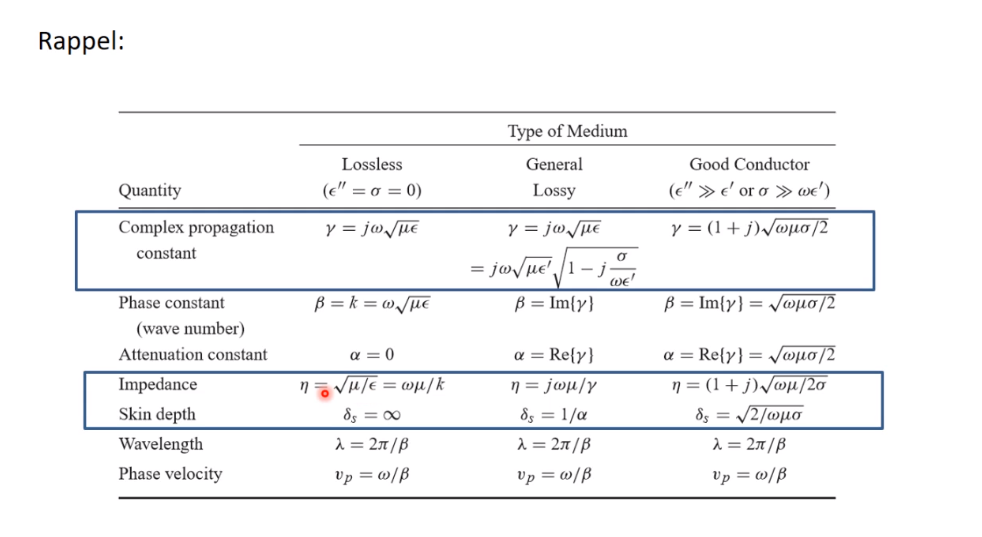
\includegraphics[scale=0.5]{tab.png}

\[
	P_l = \dfrac{\sigma |E_0|^2 |T|^2}{4\alpha}
\]

Pour un conducteur parfait : \(\sigma \rightarrow \infty\), \(T \rightarrow 0 \Rightarrow \Gamma \rightarrow -1\)

\subsection{Incidence oblique}

(Pour simplifier on se place en polarisation dans le plan (xoz))

\[
	\vec{E_i} = E_0 ( x \cos \theta_i - z \sin \theta_i) e^{-jk_1 (x\sin\theta_i + z\cos\theta_i)}
\]
\[
	\vec{H_y} = y \dfrac{E_0}{\eta_1} e^{-jk_1 (x \sin \theta_i + z\cos \theta_i)}
\]

avec \(k_1 = \omega \sqrt{\varepsilon_1 \mu_0}\) et \(\eta_1 = \sqrt{\dfrac{\mu_0}{\varepsilon_1}}\)

\chapter{Lignes de transmission et guides d'ondes}

\begin{center}
\textbf{CM10 (2021-03-25)}
\end{center}

\section{Solution générale}

Rappel, résolution de l'équation de Helmholtz dans un milieu infini :
\[
	\vec{E}(x,y,z) = \vec{E_0}e^{-\gamma z} 
\]

Pour un milieu non infini : 
\[
	\vec{E}(x,y,z) = \vec{E_0}(x,y,z)e^{-\gamma z}
\]

On simplifie en disant qu'il y a une symétrie de translation suivant (Oz), il y a donc indépendance en z.
\begin{align*}
	\vec{E}(x,y,z) &= \vec{E_0}(x,y) e^{-\gamma z} = (\vec{e}(x,y) + \text{\^z} e_z (x,y))e^{-j\beta z}
\end{align*}

Avec : \(\gamma = \alpha + j\beta \quad \beta\) constante de phase et \(\alpha=0\) l'atténuation

\[
	\vec{H}(x,y,z) = \vec{H_0}(x,y) e^{-\gamma z}= (\vec{h} (x,y) + \text{\^z} h_z (x,y))e^{-j\beta z}
\]
\(\nabla \times \vec{E} = -j\omega \mu \vec{H}\)
\[
	\left[
	\begin{array}{c}
		\dfrac{\partial E_z}{\partial y} - \dfrac{\partial E_y}{\partial z}\\\\
		\dfrac{\partial E_w}{\partial z} - \dfrac{\partial E_z}{\partial x}\\\\
		\dfrac{\partial E_y}{\partial x} - \dfrac{\partial E_x}{\partial y}
	\end{array}
	\right]
	= -j\omega \mu
	\left[
	\begin{array}{c}
		H_x\\
		H_y\\
		H_z
	\end{array}
	 \right]
\]

\(\nabla \times \vec{H} = j\omega \varepsilon \vec{E}\)
\[
	\left[
	\begin{array}{c}
		\dfrac{\partial H_z}{\partial y} - \dfrac{\partial H_y}{\partial z}\\\\
		\dfrac{\partial H_w}{\partial z} - \dfrac{\partial H_z}{\partial x}\\\\
		\dfrac{\partial H_y}{\partial x} - \dfrac{\partial H_x}{\partial y}
	\end{array}
	\right]
	= j\omega \varepsilon
	\left[
	\begin{array}{c}
		E_x\\
		E_y\\
		E_z
	\end{array}
	 \right]
\]

On a :
\[
	\left\lbrace
		\begin{array}{c}	
			\dfrac{\partial E_z}{\partial y} + \gamma E_y = -j\omega \mu H_x\\
			-\gamma E_x - \dfrac{\partial E_z}{\partial x} = -j\omega \mu H_y\\\\
			\dfrac{\partial E_y}{\partial x} - \dfrac{\partial E_x}{\partial y} = -j\omega \mu H_z
		\end{array}
	\right.
\]

\[
	\left\lbrace
		\begin{array}{c}	
			\dfrac{\partial H_z}{\partial y} + \gamma H_y = j\omega \varepsilon E_x\\
			-\gamma H_x - \dfrac{\partial H_z}{\partial x} = j\omega \varepsilon E_y\\\\
			\dfrac{\partial H_y}{\partial x} - \dfrac{\partial H_x}{\partial y} = j\omega \varepsilon E_z
		\end{array}
	\right.
\]

\[
	\Rightarrow H_x = \dfrac{1}{-j\omega \mu} \left( \dfrac{\partial E_z}{\partial y} + \gamma E_y \right)
\]
\[
	\Rightarrow E_y = \dfrac{1}{-j\omega \varepsilon} \left( -\dfrac{\partial H_z}{\partial x} - \gamma H_x \right)
\]

En posant : \(k_c^2 = \gamma^2 + \omega^2 \varepsilon \mu = \omega^2 \varepsilon \mu - \beta^2\) la fréquence de coupure :

\[
	H_x = \dfrac{j}{k_c^2}\left( \varepsilon \omega \dfrac{\partial E_z}{\partial y} - \beta \dfrac{\partial H_z}{\partial x} \right)
\]

De la même façon :
\begin{align*}
	H_x &= \dfrac{j}{k_c^2}\left( \varepsilon \omega \dfrac{\partial E_z}{\partial y} - \beta \dfrac{\partial H_z}{\partial x} \right)\\
	H_y &= \dfrac{-j}{k_c^2}\left( \varepsilon \omega \dfrac{\partial E_z}{\partial x} - \beta \dfrac{\partial H_z}{\partial y} \right)\\
	E_x &= \dfrac{-j}{k_c^2}\left( \beta \dfrac{\partial E_z}{\partial x} - \mu \omega \dfrac{\partial H_z}{\partial y} \right)\\
	E_y &= \dfrac{j}{k_c^2}\left( - \beta \dfrac{\partial E_z}{\partial y} - \mu \omega \dfrac{\partial H_z}{\partial x} \right)
\end{align*}

Nous définissons 3 modes spécifiques de propagation :

\subsection{Le mode TEM: transverse, électrique et magnétique \(E_z = H_z = 0\)}

On ne peut pas utiliser les équations précédentes car on a une division par 0 dans ce cas.
\begin{align*}
	\gamma E_y &= -j\omega \mu H_x\\
	-\gamma E_x &= -j\omega \mu H_y\\
	\dfrac{\partial E_y}{\partial x} - \dfrac{\partial E_x}{\partial y} &= 0\\
	\\
	\gamma H_y &= j\omega \varepsilon E_x\\
	-\gamma H_x &= j\omega \varepsilon E_y\\
	\dfrac{\partial H_y}{\partial x} - \dfrac{\partial H_x}{\partial y} &= 0
\end{align*}

L'équation d'Helmoltz reste la même :
\[
	\Delta \vec{E}(r,t) - \dfrac{\varepsilon \mu \partial^2 \vec{E}(r,t)}{\partial t^2} = 0
\]

On peut la transformer :
\[
	\left( \dfrac{\partial^2}{\partial x^2} + \dfrac{\partial}{\partial y^2} \right) E_x(x,y) = 0
\]

Car \(k = \beta = \omega \sqrt{\varepsilon \mu}\)

Les composantes transverse des champs ont les même propriétés que des champs E et H en électrostatique ou magnétostatique.

\paragraph{Impédance d'onde des modes TEM :} \(\vec{h} (x,y) = \dfrac{1}{Z_{TEM}} \text{\^z} \times \vec{e} (x,y)\)
\[
	Z_{TEM} = \dfrac{E_x}{H_y} = \dfrac{\omega \mu}{\beta} = \sqrt{\dfrac{\mu}{\varepsilon}} = \eta \quad \text{ Avec } \beta = k
\]

\[
	Z_{TEM} = \dfrac{-E_y}{H_x} = \sqrt{\dfrac{\mu}{\varepsilon}} = \eta \quad \text{ Impédance de la fréquence}
\]

\paragraph{Procédure pour traiter une propagation TEM :} \quad

\begin{enumerate}
	\item Trouver le potentiel V(x,y) avec des constantes inconnues
	\item Déterminer les inconnues (conditions aux limites)
	\item Trouver les composantes transverses de E
	\item  Puis de H (avec l'impédance)
\end{enumerate}

\subsection{Mode TE : pas de composante longitudinale du champ E \(E_z = 0\)}

\begin{align*}
	H_x &= \dfrac{j}{k_c^2}\left(\beta \dfrac{\partial H_z}{\partial x} \right)\\
	H_y &= \dfrac{-j}{k_c^2}\left( \beta \dfrac{\partial H_z}{\partial y} \right)\\
	E_x &= \dfrac{-j}{k_c^2}\left(\mu \omega \dfrac{\partial H_z}{\partial y} \right)\\
	E_y &= \dfrac{j}{k_c^2}\left(\mu \omega \dfrac{\partial H_z}{\partial x} \right)
\end{align*}

Dans ce cas on a \(k_c \neq 0\), pour utiliser ces relations, il faut calculer \(H_z\). On a \(k_x^2 = \gamma^2 + \omega^2 \varepsilon \mu = \omega^2 \varepsilon \mu - \beta^2\), on suppose qu'il n'y a pas de perte dans le matériau diélectrique, \(\gamma = j \beta\)

\begin{center}
\textbf{CM11 (2021-04-01)}
\end{center}

Forme de H: \(\vec{H} (x,y,z) = (\vec{h} (x,y) + \text{\^z} h_z(x,y))e^{-j\beta z}\).

Équation de Helmholtz pour la composante \(H_z\) : \(\left ( \dfrac{\partial^2}{\partial x^2} + \dfrac{\partial^2}{\partial y^2} + \dfrac{\partial^2}{\partial z^2} + k^2 \right ) H_z (x,y,z) = 0\)

Avec : \(H_z (x, y, z) = h_z(x,y) e^{-j\beta z}\)

\[
	\left ( \dfrac{\partial^2}{\partial x^2} + \dfrac{\partial^2}{\partial y^2} + k_c^2 \right ) h_z(x,y) = 0
\]

Avec \(k_c^2 = k^2 - \beta^2 = \omega^2 \varepsilon \mu - \beta^2\)

\subsubsection{Impédance d'onde des modes TE}

\[
	Z_{TE} = \dfrac{E_x}{H_y} = -\dfrac{E_y}{H_x} = \dfrac{\omega \mu }{\beta} = \dfrac{k\eta}{\beta}
\]

\subsection{Mode TM: pas de composante longitudinale du champs H (\(H_z = 0\)) }

Procédure pour traiter une propagation TE/TM:
\begin{enumerate}
	\item Résoudre l'équation de Helmhotz pour trouver \(h_z\) ou \(e_z\)
	\item Trouver les composantes transverses à partir de \(h_z\) ou \(e_z\)
	\item Appliquer les conditions aux limites
\end{enumerate}

\subsection{Pertes diélectriques pour les modes TEM et TE/TM}

\[
	\gamma = \alpha + j\beta = \sqrt{k_c^2-k^2}
\]
\[
	k^2 = \omega^2 \mu \varepsilon = \omega^2 \mu(\varepsilon' 6 j\varepsilon'') = \omega^2 \mu \varepsilon'(1-j \tan \delta )
\]

\[
	\gamma = \sqrt{k_c^2 6 \omega^2 \mu_0 \varepsilon_0 \varepsilon_r (1 6 j \tan \delta )} \quad \text{Sans magnétisme} 
\]

Avec des DL et \(\tan \delta \ll 1\) on a :
\[
	\gamma \simeq \sqrt{k_c^2 - k^2} + \dfrac{jk^2 \tan \delta}{2\sqrt{k_c^2 - k^2}}
\]

\[
	\gamma \simeq \dfrac{k^2 \tan \delta}{2\beta} + j\beta
\]

En TE et TM : \(\alpha = \dfrac{k^2\tan \delta}{2\beta}\) et en TEM \(\alpha = \dfrac{k \tan\delta}{2}\) (On a \(j\beta = \sqrt{k_c^2 - k^2}\))

\section{Guide à faces parallèles}

Guide le plus simple qui supporte les modes TE et TM, et TEM (2 électrodes). Nous nous plaçons dans le cas de matériaux métalliques parfaits, le champ électrique est nul à l'intérieur.

\subsubsection{Étude du mode TEM}

\[
	\left ( \dfrac{\partial^2}{\partial x^2} + \dfrac{\partial}{\partial y^2} \right ) V(x,y) = 0 \quad \text{ Pour } 0< x < > ; 0 < y < d
\]

En supposant un potentiel nul pour la plaque du bas, nous pouvons écrire :
\[
	V(x,0) = 0
\]
\[
	V(x,d) = V_0
\]

Du fait de la symétrie, nous n'avons pas de dépendance de V en fonction de x
\[
	V = V(y) = A + By = V_0 y/d
\]

\[
	\vec{e} = -grad V
\]

Le champ transverse s'écrit donc : \(\vec{e}(x,y) = \dfrac{-V_0}{d}\text{\^y}\)

\[
	\vec{E}(x,y,z)=\vec{e}(x,y) e^{-\gamma z} = \vec{e}(x,y) e^{-j\beta z} quad \text{ Dans un cas sans perte} 
\]

\[
	\vec{H}(x,y,z) = \vec{h}(x,y) e^{-j\beta z}
\]

\[
	\vec{H}(x,y,z) = \dfrac{1}{eta} \text{\^z} \times \vec{E}(x,y,z) = \text{\^x} \dfrac{V_0}{\eta d} e^{-j\beta z}
\]
Avec \(\beta = \omega \sqrt{\varepsilon \mu}\) et \(\eta = \sqrt{\dfrac{\varepsilon}{\mu}}\)

\subsubsection{Étude du mode TM}

Les modes TM sont caractérisés par \(H_z = 0\), et \(E_z\) différent de 0

Équation de Helmholtz pour la composante \(E_z\) : 
\[
	\left ( \dfrac{\partial}{\partial x^2} + \dfrac{\partial}{\partial y^2} + \dfrac{\partial}{\partial z^2} + k^2\right ) E_z(x,y,z) = 0
\]

Avec \(E_z (x,y,z) = e_z(x,y) e^{-j\beta z}\)

\[
	\left ( \dfrac{\partial}{\partial x^2} + \dfrac{\partial}{\partial y^2} + k_c^2\right ) e_z(x,y) = 0
\]

Ici \(e_z(x,y)\) est indépendant de x du faire de la géométrie du guide:
\[
	\left ( \dfrac{\partial}{\partial y^2} + k_c^2\right ) e_z(y) = 0
\]

\[
	e_z(y) = A \sin(k_c y) + B \cos(k_c y)
\]

Composante tangentielle à la surface continue
\[
	e_z (y) = 0 \qquad \text{À } y=0, y=d
\]

\[
	\Rightarrow \left \lbrace \begin{array}{l}
	B=0\\
	k_c = \dfrac{n\pi}{d}	
	\end{array}
	\right .
\]

\[
	e_z(y) = A_n \sin\left ( \dfrac{n\pi}{d}y\right )
\]

\[
	E_z (x,y,z) = A_n \sin\left ( \dfrac{n\pi}{d}y\right )e^{-j\beta z}
\]

\[
	\left \lbrace \begin{array}{l}
	H_x = \dfrac{j\omega \varepsilon}{k_c} A_n \cos \left (\dfrac{n\pi}{d}y\right ) e^{-j\beta z}\\
	E_y = \dfrac{-j\beta}{k_c} A_n \cos \left ( \dfrac{n\pi}{d} y \right ) e^{-j \beta z}\\
	E_x = H_y = 0
	\end{array}
	\right.
\]

Pour \(n = 0\), on a \(E_z = 0 \Rightarrow\) les champs \(E_y\) et \(H_x\) sont constants

Le mode \(TM_0\) est alors identique au mode TEM.

Pour \(n>0\) la situation est différente : chaque mode possède sa propre constante de propagation
\[
	\beta = \sqrt{k^2 - k_c^2} = \sqrt{k^2 - (n\pi/d)^2}
\]

\(\beta\) est un réel seulement quand \(k > k_c\)
\[
	k = \omega \sqrt{\varepsilon \mu}
\]
k étant proportionnel à la fréquence, il n'y aura propagation uniquement après la fréquence de coupure \(f_c\)

\[
	f_c = \dfrac{k_c}{2\pi\sqrt{\varepsilon \mu}} = \dfrac{n}{2d \sqrt{\varepsilon \mu}}
\]

La vitesse de phase : \(v_p = \dfrac{\omega}{\beta}\)

\[
	\beta = \sqrt{k^2 - k_c^2} = \sqrt{k^2 - (n\pi/d)^2}
\]
\(\beta\) devient inférieur à k, donc la vitesse de phase devient supérieur à c.

\paragraph{Impédance}\quad

\[
	Z_{TM} = \dfrac{-E_y}{H_x} = \dfrac{\beta}{\omega \varepsilon} = \dfrac{\beta \eta}{k}
\]

La puissance moyenne traversant une section transverse du guide est :
\begin{align*}
	P_{moy} &= \dfrac{1}{2} Re \int_S \vec{E} \wedge \vec{H}* \text{\^n} ds\\
	&= \dfrac{1}{2} Re \int_{w=0; y=0}^{x=W; y=d}\vec{E} \wedge \vec{H}* \text{\^z} dxdy\\
	&= \dfrac{1}{2} Re \int_{w=0; y=0}^{x=W; y=d} E_y H_x* dxdy
\end{align*}

\[
	P_{moy} =  \dfrac{WRe(\beta) \varepsilon \omega d}{2 k_c^2} |A_n|^2 \int_{y=0}^{y=d} \cos^2\left ( \dfrac{n\pi y}{d} \right ) dy
\]

Pour n > 0 
\[
	P_{moy} = \dfrac{WRe(\beta) \varepsilon \omega d}{4 k_c^2} |A_n|^2
\]
Quand n = 0
\[
	P_{moy} = \dfrac{WRe(\beta) \varepsilon \omega d}{2 k_c^2} |A_n|^2
\]

\subsubsection{Étude du mode TE}

Les modes TM sont caractérisé par \(E_z = 0\), et \(H_z\) différent de 0.

\[
	h_z(y) = A\sin(k_c y) + B \cos(k_c y)
\]

Composante tangentielle du champ électrique à la surface continue
\[
	E_x(y) = 0 \qquad \text{À} y=0, y= d
\]

Nous devons donc d'abord calculer \(E_x\).
\[
	E_x (x,y,z)= \dfrac{-j\omega \mu }{k_c} \left ( A \cos(k_c y) - B \sin (k_c y) \right ) e^{-j \beta z}
\]

\section{Les autres lignes ou guide}

Guide cylindrique et rectangulaire : pas de mode TEM

\section{Résonateurs : Cavités résonantes}

Méthode : 
\begin{enumerate}
	\item Nous partons des résultats obtenus avec deux plaques métalliques parallèles
	\item Nous rajoutons des cotés
\end{enumerate}

\subsubsection{Étude du mode TE}

Les modes TM sont caractérisés par $ E_z = 0$ et $H_z$ 

\[
	h_z (x,y) = ( A \cos(k_x x ) + B \sin (k_x x) - C \cos (k_y y) + D \sin (k_y y))
\]

\chapter{Théorie des lignes}

\section{Phénomène de propagation}

\subsection{Rappel sur les ondes : stationnarité / propagation}

Onde au niveau du générateur $ V_e(t) = V_0 \sin \omega t$

Onde en tension qui s'éloigne du générateur. $ V_e (x, t) = V_0 \sin (\omega t - \beta x)$ avec $ \beta = $ contante de propagation $ = \omega / v$ avec $v$ la vitesse de l'onde.

Si $L \ll \lambda$ courants constants quel que soit x (à to donné) régime stationnaire

Si $L \gg \lambda$ variation de courant suivant x, propagation.

\paragraph{Exemple} calculer $\lambda$ pour :

Le réseau EDF, $f = 50Hz$

Circuit électronique basse fréquence ( 1 MHz)

Circuit haute fréquence (10 GHz) problème de périodicité spatiale

Avec c = $3 \E{8} ms^{-1}$

\subsection{Équation des télégraphistes}

\subsubsection{Courants quasi-stationnaires}

Si on décompose une ligne de grande longueur (l)en segments de longueur dx telle que $dx \ll l$. On peut alors considérer des courants quasi-stationnaires.

\section{Équation des télégraphistes}

\[
	\dfrac{\partial i(x,t)}{\partial x} = - G \cdot v(x,t) - C \cdot \dfrac{\partial v(x,t)}{\partial t}
\]

\paragraph{Équation des télégraphistes}

\[
	\dfrac{\partial^2 v(x,t)}{\partial x^2} = LC \dfrac{\partial^2 (v(x,t)}{\partial t^2} + (RC + LG) \dfrac{\partial v(x,t)}{\partial t} + RG \cdot v(x,t)
\]
\[
	\dfrac{\partial^2 i(x,t)}{\partial x^2} = LC \dfrac{\partial^2 i(x,t)}{\partial t^2} + (RC + LG) \dfrac{\partial i(x,t)}{\partial t} + RG \cdot i(x,t)
\]

Dans le cas d'une ligne sans pertes, il n'y a pas de résistance ni de conductance, \(R=G = 0\)

\[
	\dfrac{\partial^2 v(x,t)}{\partial x^2} = LC \dfrac{\partial^2 v(x,t)}{\partial t^2}
\]
\[
	\dfrac{\partial^2 i(x,t)}{\partial x^2} = LC \dfrac{\partial^2 i(x,t)}{\partial t^2}
\]

Équation de propagation/ équation de d'Alembert (avec \(LC = 1/v^2 \))

Équation générale de l'équation :

Somme de fonctions à une variable prise en \(t - x/v\) et \(t + x/v\)

\[
	V(x,t) = f(t-x/v) + g(t+x/v)
\]
Somme d'une onde progressive et d'une onde réfléchie.

\subsubsection{Impédance caractéristique}

\[
	Z_C = \sqrt{\dfrac{R + jL\omega}{G + jC\omega}}
\]

Dans le cas de la ligne sans perte, \(R=G=0\)
\[
	Z_C = \sqrt{\dfrac{L}{C}}
\]

\subsubsection{Calcul de l'impédance rapportée en x, Z(x)}

\[
	\underline{V(x)} = \underline{V}_i \cdot e^{-\gamma x} + \underline{V}_r \cdot e^{\gamma x} \qquad  \underline{I(x)} = \underline{I}_i \cdot e^{-\gamma x} + \underline{I}_r \cdot e^{\gamma x}
\]

En posant \(Z_0 = \dfrac{\underline{V(0)}}{\underline{I(0)}}\)
\[
	\Rightarrow Z(x) = Z_C \dfrac{Z_0 - Z_c \cdot \tanh(\gamma x)}{Z_C - Z_0 \cdot \tanh (\gamma x)}
\]

\subsubsection{Cas : \(Z_r = Z_C\) (Impédance de charge = impédance caractéristique)}

\[
	Z_0 = Z_C
\]
\[
	Z_0 =  \dfrac{\underline{V(0)}}{\underline{I(0)}} = Z_C
\]
\[
	\underline{V}_i = \underline{V}(0) \qquad \underline{V}_r = 0 \qquad \text{Pas de reflexion}
\]

\subsubsection{Cas \(Z_r = 0\)}
\begin{center}

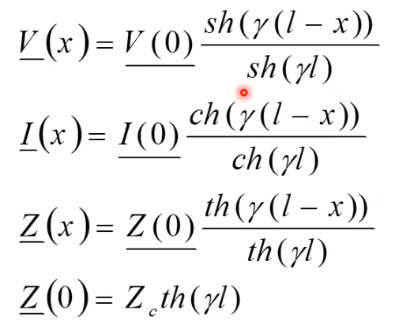
\includegraphics[scale=0.5]{equa.png}

\end{center}

\end{document}